%%%%%%%%%%%%%%%%%%%%%%%%%%%%%%%%%%%%
% This is root file of the thesis. %
%%%%%%%%%%%%%%%%%%%%%%%%%%%%%%%%%%%%

\documentclass[11pt,a4paper,twoside]{thesis}
%\documentclass[11pt,a4paper,]{thesis}
\usepackage{amssymb}
\usepackage{amsbsy}
\usepackage{amsmath}
\usepackage{amsthm} % This is only for theorem and proofs.
\usepackage{setspace}
\usepackage{listings}
\usepackage{afterpage}
\usepackage{courier}
\usepackage{breakurl}
\usepackage[a4paper]{geometry}
\usepackage{tabu}
\usepackage{tabulary}
\usepackage{ifpdf}
\usepackage{rotating}
\usepackage{float}
\usepackage{subfig}
\ifpdf
\usepackage[disable]{todonotes}
\else
\usepackage{graphicx}
\usepackage{todonotes}
\fi
\usepackage{cite}

\title{*Template for MSc Thesis, Imperial College London*}
\author{James Rose}


%%%%%%%%%%%%%%%%%%%%%%%%%%%%%%%%%%%%
% including page setting & fancyhdr.
\setlength{\textwidth}{500pt}
\addtolength{\hoffset}{-20pt}
\setlength{\textheight}{650pt}
\setlength{\headsep}{30pt}

% Set left margin - The default is 1 inch.
\setlength{\oddsidemargin}{2cm}

% Set width of the text - What is left will be the right margin.
\setlength{\textwidth}{15cm} %5.7in

% Set top margin - The default is 1 inch
\setlength{\topmargin}{-1.5cm}

% Set height of the header
\setlength{\headheight}{1.2cm}

% Set vertical distance between the header and the text
\setlength{\headsep}{1.2cm}

% Set height of the text
\setlength{\textheight}{23cm} %9in

% Set vertical distance between the text and the
% bottom of footer
\setlength{\footskip}{0.4cm}

% set belowcaptionskip.
\addtolength{\belowcaptionskip}{2ex}

%\setlength{\parindent}{2em}
\setlength{\parindent}{0pt}
%%%%%%%%%%%%%%%%%%%%%
\usepackage{fancyhdr}

\pagestyle{fancy}

\renewcommand{\chaptermark}[1]{\markright{\thechapter.\ #1}}
\renewcommand{\sectionmark}[1]{\markright{\thesection\ #1}}
\fancyhf{}
\fancyhead[LE,RO]{\bfseries\thepage}
\fancyhead[LO]{\bfseries\rightmark}
\fancyhead[RE]{\bfseries\leftmark}
\renewcommand{\headrulewidth}{0.5pt}
\renewcommand{\footrulewidth}{0pt}
\addtolength{\headheight}{0.5pt}
\fancypagestyle{plain}{
  \fancyhead[LE,RO]{\bfseries\thepage}
  \fancyhead[LO]{}
  \fancyhead[RE]{}
  \renewcommand{\headrulewidth}{0.5pt}
} 

\def\mystretch{1.5}

\newlength{\figX}
\newlength{\figY}
\newlength{\tmplen}

\newlength{\matFigX}
\newlength{\matFigY}

\setlength{\matFigX}{4.04in} \setlength{\matFigY}{3.04in}

\setlength{\parindent}{0pt}
\setlength{\parskip}{1ex}
\setlength{\parindent}{3em}
\sloppy

\hyphenation{another}

%%%%%%%%%%%%%%%%%%%%%%%%%%%%%%%%%%%
% The Beginning of a LaTeX document
\begin{document}

%%%%%%%%%%%%%%%%%%%%%%%%%%%%%%%%
% The Cover Page of PhD Thesis %
%%%%%%%%%%%%%%%%%%%%%%%%%%%%%%%%
\thispagestyle{empty}

\begin{center}
\null \vspace{\stretch{0.2}}
\renewcommand{\baselinestretch}{2}
\doublespacing
\textsc{\huge{An FPGA Cluster for Real-Time \vspace{\stretch{1}} Parallel Human Genome Assembly}}



\vspace{\stretch{1}}
\textsc{\large{J C Rose}} \\
\textsc{\large{Supervisor: Dr. P Georgiou}} \\
\textsc{\large{2nd Marker: Prof. C Toumazou}} 
\vspace{\stretch{1}}

\vspace{\stretch{1}}
A Thesis submitted in fulfilment of requirements for the degree of \\
Master of Engineering of Imperial College London
\vspace{\stretch{1}}
%\centerline{\special{bmp:ic.bmp x=2cm}}
%\centerline{\hbox to 2cm{\epsfig{file=ic.eps,width=2cm,clip=}}}


\vspace{\stretch{0.1}}


Department of Electrical and Electronic Engineering\\
Imperial College London\\
June 20\textsuperscript{th}, 2013
\end{center}




%%%%%%%%%%%%%
\onehalfspacing

\frontmatter
\setlength{\tmplen}{\parskip}
\setlength{\parskip}{-1ex}
 
\renewcommand{\baselinestretch}{1.5}
\chapter{Abstract}
\renewcommand{\baselinestretch}{\mystretch}

%\setlength{\parindent}{2em}

Presented in this report is a practical implementation of a scalable comparison engine algorithm for use in a DNA sequencing toolchain. Having shown all-against-all comparison to be a key computational problem in DNA sequencing for short read Next Generation Sequencing, an algorithm designed by Y Hu has been presented as a possible solution. This algorithm was modified and implemented in VHDL for use across a multi-device cluster for the purpose of speeding up comparison through the use of parallelism. The design was implemented on a proof of concept machine consisting of 3 small FPGAs, capable of comparing 27 sequences of any practical length in parallel. A key aim of the project was to minimise any overhead in inter-device communication and this was achieved with only a 2 clock cycle per comparison  increase. A shared clock design was utilised with clock speed maintained at 33.1MHz while scaling across multiple FPGAs with performance unaffected by inter-device communication. Logic overhead introduced by the modifications used up to 4,000 logic elements per device, a minor increase in the total size of the algorithm for large applications. Total performance metrics indicated scaling across 3 FPGAs increased performance to allow 3 times the number of comparisons in parallel whilst retaining 80\% of the comparison speed per processing element. Testing showed the cluster took $42{\mu}s$ per comparison.  A number of further modifications to the algorithm were also suggested to increase performance with minimal cost.

 \renewcommand{\baselinestretch}{1.5}
\chapter{Acknowledgments}
\markright{Acknowledgments}
\renewcommand{\baselinestretch}{\mystretch}

%\setlength{\parindent}{2em}
\onehalfspacing
I would like to thank Dr Georgiou for his continued support and advice throughout the project, particularly in relation to the biomedical engineering aspects of this project. I would also like to that Professor Toumazou for his advice early in the project. Finally, I would like to the acknowledge Yuanqi Hu whose support has been invaluable in developing this project and without whom there would have been no basis for this project.
 \doublespacing
 \tableofcontents
 \listoffigures
\onehalfspacing

% \listoftables
\renewcommand{\baselinestretch}{\mystretch}
% \renewcommand{\baselinestretch}{1}
\chapter{Abbreviations}
\markright{Abbreviations}

\begin{tabular}{rl}
  \vspace{0.1em} \textbf{TLA:} & Three Letter Abbreviation \\
  \vspace{0.1em} \textbf{OA:} & Other Abbreviation\\
\end{tabular}



\setlength{\parskip}{\tmplen}
%%%%%%%%%%%%
\mainmatter
\fancyhead[RE]{\emph{Chapter \thechapter}}
\renewcommand{\baselinestretch}{\mystretch}
% Use \input to include your chapters as illustrated below
\chapter{Introduction}
\renewcommand{\baselinestretch}{\mystretch}
\label{chap:Intro}
The last 25 years have seen an ever-increasing demand for fast and efficient Deoxyribonucleic Acid (DNA) sequencing with the development of the field of genomics and large projects such as The Human Genome Project. Practical applications of DNA sequencing have grown massively with sequencing becoming an important technology in fields as diverse as medicine and ecology. As well as growth in the applications of sequencing, there have been significant advances in the technology used. Next Generation Sequencing (NGS) technologies have increased the speed at which sequencing can occur through new parallel technology with high speed digital processing back-ends. These newer sequencing techniques can produce data sets of the order of billions of base pairs; which places requirements on the digital signal processing technologies that form a critical part of the sequencing tool chain.


The NGS technologies that have been developed place restrictions on the how DNA can be efficiently detected and sequenced. The pyrosequencing technology that is commonly used to detect the bases that form the sequence of DNA can be scaled well to small detector sizes and packed relatively densely, fitting up to 1 million pixels on a single chip. The limitation of these methods however, is that they are relatively slow with each base taking up to 4 seconds to detect \cite{rothberg2011integrated}. As a result the only way to sequence long DNA patterns is to split them into smaller sub-sequences for detection. This leaves a problem to be solved in the digital processing back-end of the sequencer \cite{shendure2008next}. The resultant data is a large number of short sequences, the order of which is unknown. In order to overcome this signal processing problem a comparison engine is required to detect overlaps in the sequences and produce a profile of the data which can then be used to repair the sub-sequences into one full sequence. 


In this report a novel method of DNA sub-sequence assembly will be introduced. Based on the algorithm produced by Y Hu et al. a scalable Field Programmable Gate Array (FPGA) cluster will be developed with the intention of speeding up the DNA sequencing process to the point where real-time DNA sequencing is possible. The design will be motivated by the specific properties of modern NGS systems and will be specified in a manner that allows it to be dropped in to a tool-chain with minimal adaptation. Within this project an example cluster will be developed and robustly tested as a proof of concept, while algorithms will be designed to allow for maximal scalability. Testing will be used to quantify the power of the system at given specifications and compared to both the original simulated algorithm by Y Hu and other available algorithms.


\section{Aims and Objectives}
The primary aim of this project is to modify an existing comparison engine algorithm to map onto a cluster of FPGAs. This involves designing a custom hardware set up of multiple interconnected devices suitable for off-loading the computationally expensive DNA sequence comparison. The key deliverable from this objective will be a framework of FPGA hardware, Hardware Description Language (HDL) code, and Host interface software. This will be accompanied by a user guide attached to this report as appendix \ref{App:UserGuide}. The evaluation of whether this objective has been achieved will be covered in the testing section with a set of tests to confirm the operation of the system as well as evaluating its functionality performance towards the key aim of being a real-time solution.

As a sub-objective, the design delivered for the primary goal should be structured such that it can be easily implemented on alternative hardware applications for different scales of problem size. Efficiency and performance are key metrics of success in the project and these will be evaluated in chapter \ref{chap:evaluation} using both simulated result for the adopted algorithm as well as other algorithms discussed in the related work section. The real-time nature of the system will be discussed and any limiting factors should be identified.


Part of the objective of the system is its performance is comparable with that of current solutions, particularly in comparison to the freely available sequencing tools available such as ABySS. This objective will be evaluated through tests comparing the algorithm with software solutions introduced in the related work section.

\pagebreak
\section{Report Structure}
Chapter two of this report introduces the area of DNA sequencing, and the tools that are used. In particular it introduces a comparison engine algorithm that will be adopted to speed up the sequencing process and analyses the scalability of this algorithm respect to different parameters. 

Chapter three looks at the different techniques currently being developed in DNA sequencing and FPGA based design. Particular emphasis will be placed on FPGA based comparison engine algorithms and any techniques they use that could be adopted as part of this project. 

Chapter four describes the important design aspects of this project, focusing on areas of particular complexity and interest. Split between the hardware setup, algorithmic implementation and host computer based interface. This section comprises the bulk of the new work presented in this report.

Chapter five covers any challenges that were met when transferring the design from simulation to application and the limitations these problems may introduce on scalability of the project. The majority of this section focuses on the issues encountered in a shared clock system.

Chapter six details a number of methods of testing the project, using simulation and real-world tests. Presenting both the raw data of results and graphed details of important variables and cost functions. 

Chapter 7 evaluates the test data in terms of the existing work in the area and the code the project was based on, conclusions will be drawn on how the algorithm would scale to other implementations and how this could be achieved. 

Chapter 8 expands upon the conclusions of the evaluation, suggesting possible further modifications that could be implemented to further improve the algorithm and the problem sizes this algorithm can process.

Chapter 9 finally summarises the conclusions from the project, giving the key performance metrics and revisits the aims and objectives giving a summary of to what extent each was met. %Intro
\chapter{Background and Motivation}
\renewcommand{\baselinestretch}{\mystretch}
\label{chap:bg}
%\setlength{\parindent}{0pt}



\section{Applications of DNA Sequencing}
There are a large number of motivations for sequencing DNA. In the medical field, genomics has applications in both research and applied medicine. One example where DNA sequencing has been used productively in applied medicine is for screening for the BRCA mutations. Through testing the BRCA1 and BRCA2 genes for mutations, it is possible to accurately predict if a patient is likely to develop cancer later in life. The US Preventative Services Task Force currently recommends screenings for women who are known to have a family history of breast cancer, around 2\% of the population \cite{USPSTF}. This type of application relies on exome sequencing, where only a small subsection of DNA is sampled to identify a risk factor for a certain disease. 

The research applications of sequencing have been clear for some time with  the Human Genome Project launching in 1990 \cite{HGP}.  With it's primary goals accomplished in 2003, this project has opened numerous areas for research, showing possible applications such as understanding genotypes of viruses for targeted treatments and also the advancement of other less related areas such as forensics. The sequencing of a full human genome also has significant impact on the nature of DNA sequencing, as it allows a much wider area of mapping sequencing. Mapping sequencing uses the fact that the structure of a piece of DNA is known in order to simplify the sequencing process. Exome sampling mentioned earlier is an example of this. 

DNA sequencing also plays an important role in ecology research where bio-diversity and historical biological characteristics can both be indicated by DNA samples and used to further current research. This field is particularly cost sensitive due to the enormous variety of DNA sampling that needs to be carried out and also presents some of the most complex problems for DNA sampling \cite{genomelength}.An example of this is the Polychaos Dubium which has 670 Giga base pairs (Gbp), dwarfing the size of the human genome at 3Gbp \cite{HGP2}. Due to the complexity of the operations we will see in the DNA sequencing process this presents important problems in sequencing \cite{parfrey2008dynamic}. Often this area often requires de novo sequencing techniques, using no prior knowledge of the genome in contrast to human samples where the general structure of the genome is known and can be used to simplify sequencing.  These de novo techniques present a significantly different problem set to exome sequencing where comparison against existing data is impossible.


Ecology research has significant practical applications within agriculture, where studies such as the sequencing of the Oil Palm genome are currently being undertaken in order to identify important genetic traits such as drought resistance and yield. It is in areas like these where fast sequencing of particularly long genetic sequences have practical applications, which acts as a driving motivation for producing a scalable architecture for this problem. Genetically Modified Organisms (GMO) are currently a growing trend in agriculture, with some companies in this area yielding over \$2Billion operating income per year \cite{Monsanto}.

In order to satisfy the growing demand for both full de novo sequencing and exome sequencing, there has been a large amount of research in the area. The result of this research is a large array of techniques and technologies designed to lower the cost and raise the speed of sequencing. In the last decade this has produced a significant advance with a set of Next Generation Sequencing technologies.




\section{The DNA Sequencing Process}
\subsection{The Structure of DNA}
Deoxyribonucleic acid is a molecule formed of four nucleotides (guanine, adenine, thymine, and cytosine), the structure of the molecule is a double helix with bonds formed between complementary pairs of nucleotides (guanine bonding with cytosine, adenine bonding with thymine) \cite{mandelkern1981dimensions}. These bonds are referred to as base pairs (bps) and are commonly used to quantify the size of the molecule. For example, the human genome is 3 billion base pairs long. The structure of DNA tends to be extremely long sequences. This structure has important ramifications on the sequencing techniques as discussed below.
\begin{figure}[h]
  \centering
  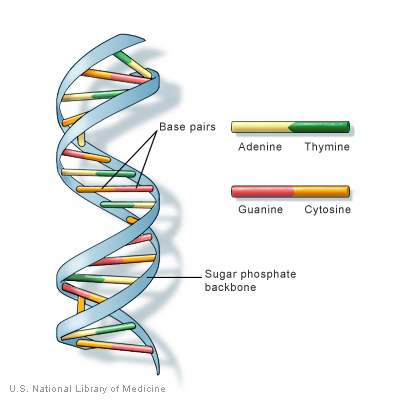
\includegraphics[width=0.45\textwidth]{./figs/dnastructure.jpg}
  \caption{The Structure of DNA \cite{USLoM}}
  \label{fig:pyro}
\end{figure}



\subsection{DNA Detection Technologies}
One of the most commonly used DNA sequencing technologies is pyroseqeuncing, with commercial tools already in use such as the Roche GS20 sequencer \cite{huse2007accuracy}. Pyrosequencing is a synthesis method, this means that the method involves recombining a single strand of DNA with it's complementary base pairs. The full process requires a double helix of DNA first to be split into 2 single strands. Once this is done, one of the strands is taken and used to recombine to the full double helix. This involves the use of a primer, containing the four nucleotides in a sequence being introduced along the single strand. When one of the bases in the primer interacts with its complementary pairing a reaction occurs. If a base repeats consecutively, the reaction occurs twice and the byproducts of the reaction are magnified in amplitude. An example of this process is shown in figure \ref{fig:pyro}.


\begin{figure}[h]
  \centering
  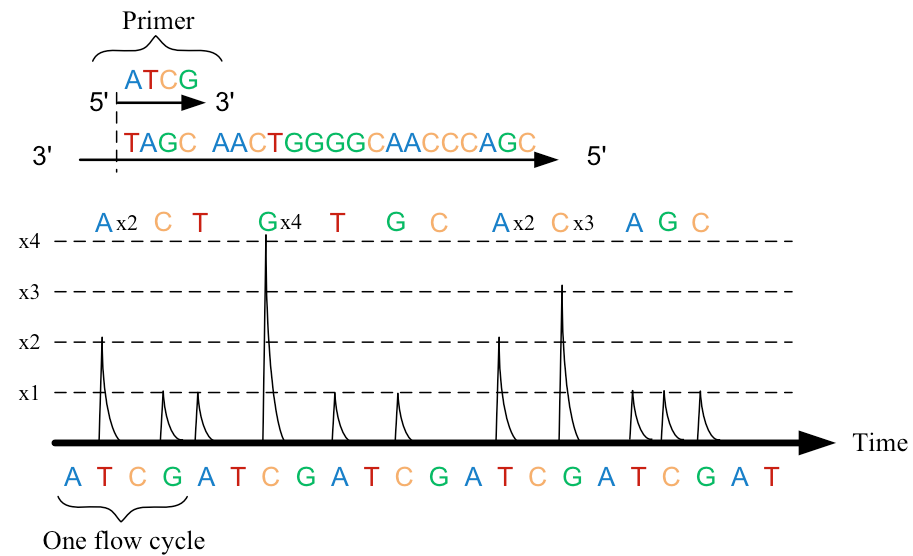
\includegraphics[width=0.75\textwidth]{./figs/pyrosequencing.png}
  \caption{Pyrosequencing, Diagram by Y Hu \cite{hu2012cmos}}
  \label{fig:pyro}
\end{figure}
This reaction releases both pyrophosphate and a positively charged hydrogen ion. In some approaches the pyrophosphate is detected using optical methods and the timing of the reaction could be used to identify which base. In newer technologies such as that introduced by Rothberg in 2011, non-optical techniques have been developed which allow much denser packing of detectors on a single chip \cite{rothberg2011integrated}. These techniques use transistor technologies called ion-sensitive field-effect transistors (ISFETS). These ISFET devices can sense a change in the pH of a surrounding solution, the pH of the solution fluctuates when a recombination of a base with its complementary pair happens. The change in pH is sensed by the ISFET and as the supplied base is known, the base in the sequence can be identified \cite{wong2010pg}.


The advantage of methods such as these is the density of detectors, allowing massively parallel sequencing to take place, Rothberg's application had 1.2 million wells on a single chip, each able to detect a nucleotide in parallel. The disadvantage of this system however, is the detection time. The synthesis process involves the introduction of chemicals to the DNA sequence and then for a reaction to occur and the resultant chemicals to reach the detector. This is relatively slow process, taking up to 4 seconds for a single detection cycle to occur \cite{rothberg2011integrated}. As a result, any practical application of this approach would need to use a massively parallel short read length approach. Due to this fact, a chemical process has been adopted to duplicate the DNA multiple times, cut it into small chunks and then use the overlaps of these chunks to recombine the sub-sequences into the full sequence. All NGS technologies share this limitation of read lengths being orders of magnitude shorter than even the shortest genome \cite{miller2010assembly}. This is not a trivial computational problem and a variety of assembly algorithms have been proposed as a solution to this. 


\subsection{Assembly Algorithms}

The problem of recombining sub-sequences into a single full sequence is computationally expensive as all overlaps of a sequence must be identified. A number of methods have been used for this, however there are three main groups. 


The Overlap-Layout-Concensus (OLC) algorithm does an all against all comparison of the sub-sequences and produces a graph of where the sequences overlap, a graph can then be produced organising the sub-sequences into order by how they overlap, at this point it is relatively computationally simple to produce a best-guess full sequence. With enough data it is possible to confidently produce a full sequence that is known to be correct. This method is computational expensive due to the all-against-all comparison required at the beginning of the process. Once the comparison is done, the recombination is a relatively trivial problem to solve. 



The Greedy Graph algorithm shares the first step with the OLC method, using an all-against-all comparison to build a graph to be solved. The disadvantage of the Greedy algorithm however, is that at each stage it picks a locally optimal solution, this means that the order of detection can determine the likelihood getting a given result \cite{hu2012cmos}. 



A significantly different approach to assembly is the De Bruijn method. Used in the Solexa and SOLiD platforms \cite{miller2010assembly}, it produces a graph of sequences where each sequence is a node on the graph and any overlaps above a threshold are directed links on the graph. The advantage of this system is that it does not require the same all against all comparison, as overlaps are built up iteratively, however due to the fact the algorithm srotes a large amount of data on sub-sequences it uses a large amount of memory relative to the other algorithms. 


The problem of assembly algorithms is therefore a matter of both approach and implementation. It is difficult however, to minimise the problem of memory usage in the De Bruijn graph assembly method. The all-against-all comparison is computationally intensive, and in this report a method will be introduced to alleviate these constraints, and attempt to scale an OLC method to produce a real-time sequencer. The method that will be used in this report was introduced by Y Hu et al. in 2012, exploiting parallelism and the detection method to produce a real-time all-against-all comparison engine \cite{hu2012cmos}.
\section{The Comparison Engine}
The comparison engine designed by Y Hu et al. looks to exploit the slow read times of the current DNA detection technologies as well as mitigating the computational complexity of the algorithm through the use of parallelism \cite{hu2012cmos}. The comparison engine works on the principle of a ring network as shown in figure \ref{fig:CE}. The system is comprised of a large number of comparator elements known as pixels. These pixels correspond to the detection pixels from the dense parallel detection technology discussed above. They are specifically designed to work on incomplete data sets in order to maximise the processing that can be completed whilst the DNA detection is still taking place. 
  
Each comparator element gets a single sequence of data fed into it from a data source, it caches this data locally. Once enough data has been cached it starts forwarding the end of this sequence to the next pixel. Each pixel then has its locally cached data and an input sequence from the previous pixel. A comparison is done between these two peices of data and the result is stored in a local overlap library. This overlap library stores all the important data to identify an overlap including the length of the overlap and the sequences which overlap. The accumulation of all the pixels' local libraries form a full overlap database which can be used to form a graph in the Overlap-Layout-Concensus algorithm.


As an extension to this basic algorithm Y Hu designed the individual pixels such that the forwarding ring can forward a compile time modifiable number of strings. For example, when setting the \verb|FIX_LENGTH| parameter to 4, each pixel forwards four sequences to the next pixel in parallel and therefore does 4 comparisons per cycle locally. The advantage of this technique is that a balance can be struck between the number of cycle required to do all the comparisons and the complexity of the local pixel. The structure of this algorithm can be seen in figure \ref{fig:CE}. 

This algorithm was provided in the form of a VHDL project, written to 1993 specification VHDL in a set of several parameterisable modules. It is important to note in this design the data source provided is un-synthesizable, this means that while it is written in VHDL similarly to the rest of the code, however it cannot be implemented on hardware. This is appropriate for simulation but not for any practical application. A key part of any practical implementation would be to replace this block with an interface to allow communication with a data source.

This designs exploits the advantages of parallelism as well as the streaming data source in this application, but a full analysis of its computational complexity must be performed to identify the possible applications of this algorithm. A large amount of this work has been quantified by Y Hu et al in a previous paper \cite{hu2012cmos} . In the following section I perform a simple analysis of the properties of this implementation in terms of its resource requirements on hardware as well as the speed and computation it is capable of doing assuming perfect availability of data and a clock speed that can be set.

\begin{figure}[h]
  \centering
  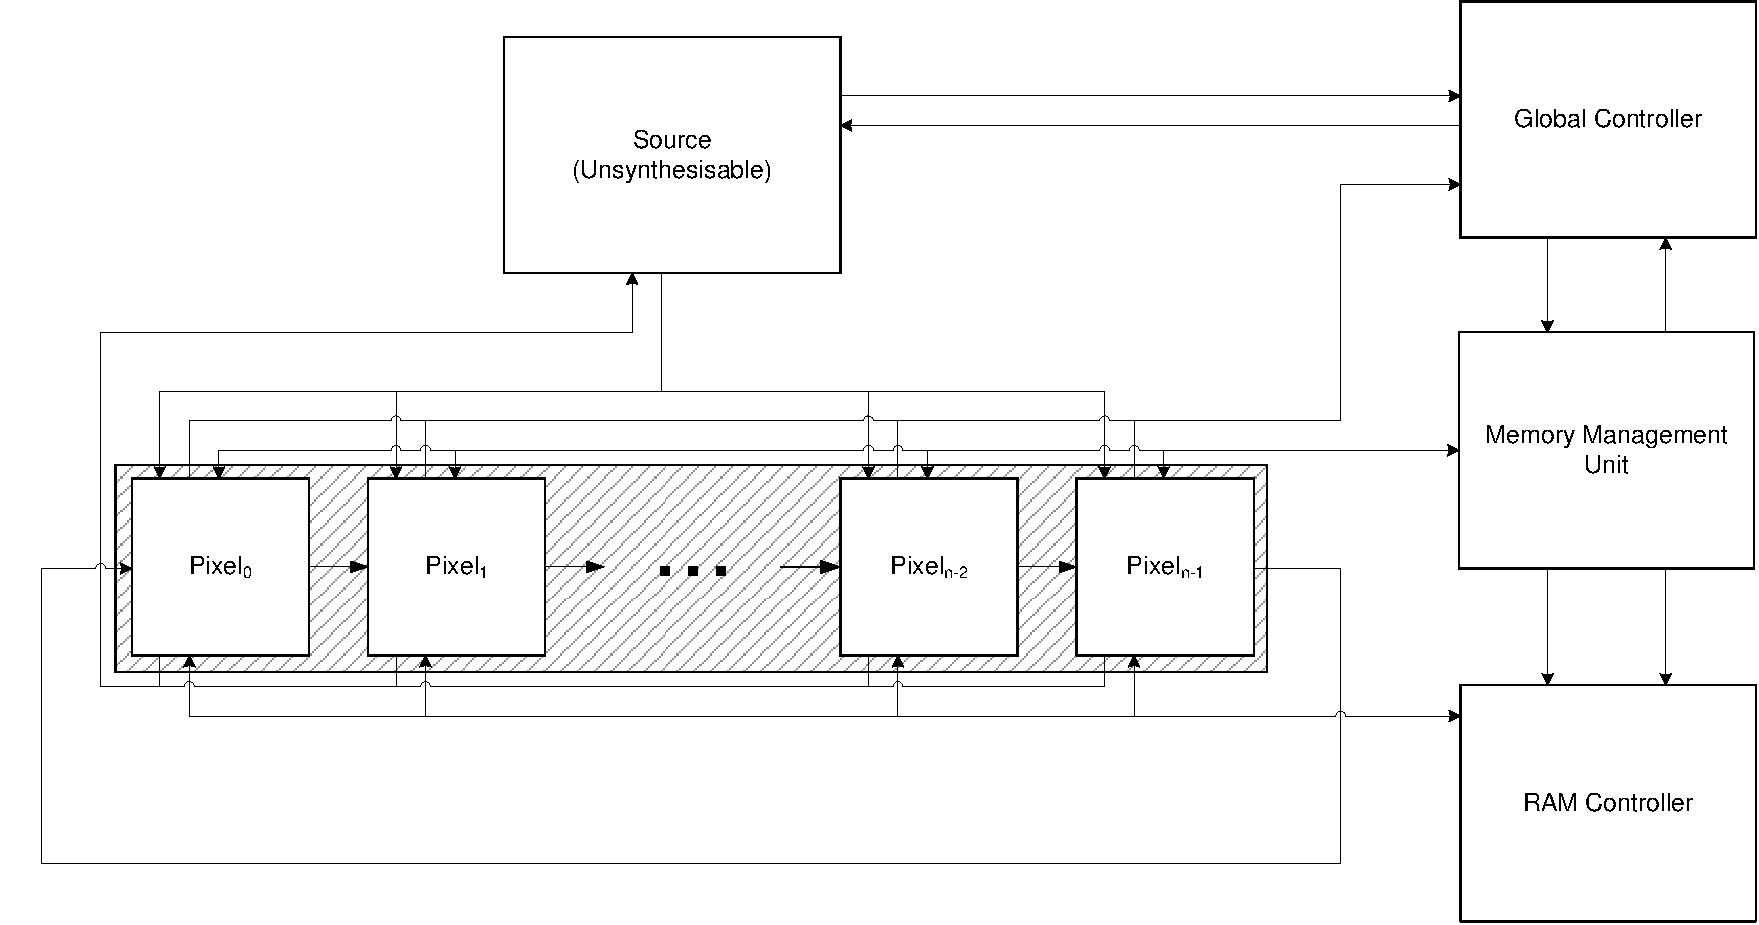
\includegraphics[width=\textwidth]{./figs/UnModified.pdf}
  \caption{Y Hu's Comparison Engine}
  \label{fig:CE}
\end{figure}

\subsection{Complexity Analysis}
The comparison engine algorithm was made available as a VHDL project that fully works in simulation with an included test bench that verifies its functionality. The VHDL implementation provided is a parameterisable project, allowing it to scale with various requirements such as read length, number of pixels and result library size. To give an idea of the scale of the code provided, a set of compilations has been run at different settings. Design size will be listed with 3 factors; Clock frequency shows the speed of design achievable, memory utilisation and logic utilisation show the size of the design.



\begin{table}[!h]
\centering % used for centering table
\begin{tabulary}{\textwidth}{C C C C| C C C}% centered columns (4 columns)
\hline\hline %inserts double horizontal lines
Read Length & Genome Length & Pixel Count & Library Size & Logic Utilisation & Memory Utilisation (Bits) & Frequency (MHz)\\      % inserts table 
%heading
\hline % inserts single horizontal line
50 & 100 & 9 & 3 & 9,916 & 4,096 & 38.5\\ % inserting body of the table
50 & 100 & 9 & 5 & 10,597 & 4,096 & 39.7\\ % inserting body of the table
50 & 100 & 9 & 7 & 11,295 & 4,096 & 39.6 \\ % inserting body of the table
50 & 100 & 9 & 10 & 12,324 & 4,096 & 40.6\\ % inserting body of the table
\hline
50 & 200 & 5 & 5 & 5,896 & 4,096 & 40.2 \\ % inserting body of the table
50 & 200 & 10 & 5 & 11,744 & 4,096 & 40.1\\ % inserting body of the table
50 & 200 & 20 & 5 & 23,590 & 4,096 & 39.5 \\ % inserting body of the table
50 & 200 & 40 & 5 & 50,513 & 4,096 & 34.1\\ % inserting body of the table
\hline
50 & 100 & 5 & 5 & 5,896 & 4,096 & 40.2\\ % inserting body of the table
50 & 1,000 & 5 & 5 & 5,896 & 4,096 & 40.2\\ % inserting body of the table
50 & 10,000 & 5 & 5 & 5,896 & 4,096 & 40.2\\ % inserting body of the table
\hline
100 & 2,000 & 5 & 5 & 5,957  & 4,096 & 41.7\\ % inserting body of the table
200 & 2,000 & 5 & 5 & 6,005 & 4,096 & 41.6\\ % inserting body of the table
400 & 2,000 & 5 & 5 & 6,047 & 4,096 & 41.6\\ % inserting body of the table
800 & 2,000 & 5 & 5 & 6,067 & 4,096 & 41.7\\ % inserting body of the table
1,600 & 2,000 & 5 & 5 & 6,110 & 4,096 & 41.7 \\ % inserting body of the table

\hline
\end{tabulary}
\caption{Design Size of Y Hu's Comparison Engine} % title of Table
\label{table:alg}
\end{table}

These measurements were made on an Altera CYCLONE III device, which is representative of the devices that this algorithm may be built on. As can be seen, logic size primarily scales with pixel count. The overlap library size also has a large effect which is associated with the ratio of read length to genome length as the more reads within the genome will cause more overlaps. Other variables have a much more limited change; the memory utilisation stays constant, as does the frequency. This is because the longest path in the design is held within a single pixel. 


In terms of absolute resources the control logic has very little overhead and the memory utilisation is very low. For any given FPGA, memory generally outnumbers logic elements significantly. In this design, the memory utilisation is very low however, and a fixed level so in this design the logic utilisation will be the limiting factor when fitting the algorithm on to a device.

\section{Hardware Acceleration}

The scope of this project was to build an FPGA accelerator for the comparison process, the reason for the choice of FPGA as the hardware for this project is several fold. The first and most important motivating factor is the reconfigurability of FPGAs, these devices are designed to be reprogrammed many times, allowing the DNA detection hardware to drive the configuration of the comparison engine. This is important due to the many possible ways the DNA detection could be done and the paralellisation of the task. The hardware for this project must also be highly parallelisable in order to take advantage of the pixel based design, a traditional central processing unit (CPU) is by nature serial and therefore could not accelerate the process in the same way. 

General purpose Graphics Processing Units (GPUs) were an alternative to FPGAs in terms of parallelisation, however these are generally not used as stand alone devices and communication between processing units in a GPU can be relatively expensive in terms of performance due the design of the GPU and the hierarchical nature of it's scheduling. Fitting the algorithm to different streaming multi-processors in a GPU would be a necessary complication of that approach. GPUs also have very limited scope for acceleration using additional hardware without complex cluster designs, communicating via protocols such as PCI-Express and this does not favour a ring network design that was discussed earlier. It is expected that FPGA development is a longer process, however the FPGA hardware is tailored perfectly to support the ring network design, allowing massive parallelisation and communication. The FPGA device is also normally a standalone device allowing it to communicate directly with the DNA  detection hardware rather than incurring the cost and delay of a host computer.


The primary motivation for using an FPGA is therefore speed, it has been shown in several papers that FPGAs are capable of signficantly speeding up parallel processess\cite{Fowers:2012:PEC:2145694.2145704}. For suitably parallel applications with large enough problem sizes FPGAs have been shown to be the best solution in terms of performance. This can be seen in figure \ref{fig:cpugpufpga} where for Sum of Absolute Differences (SAD), convolution and Correntropy the FPGA significantly outperforms CPUs and GPUs for most problems\cite{Fowers:2012:PEC:2145694.2145704}. Shown below green represents FPGA, light blue represents GPU accelerated, red represents basic GPU, and dark blue represents CPU.

\begin{figure}[h]
  \centering
  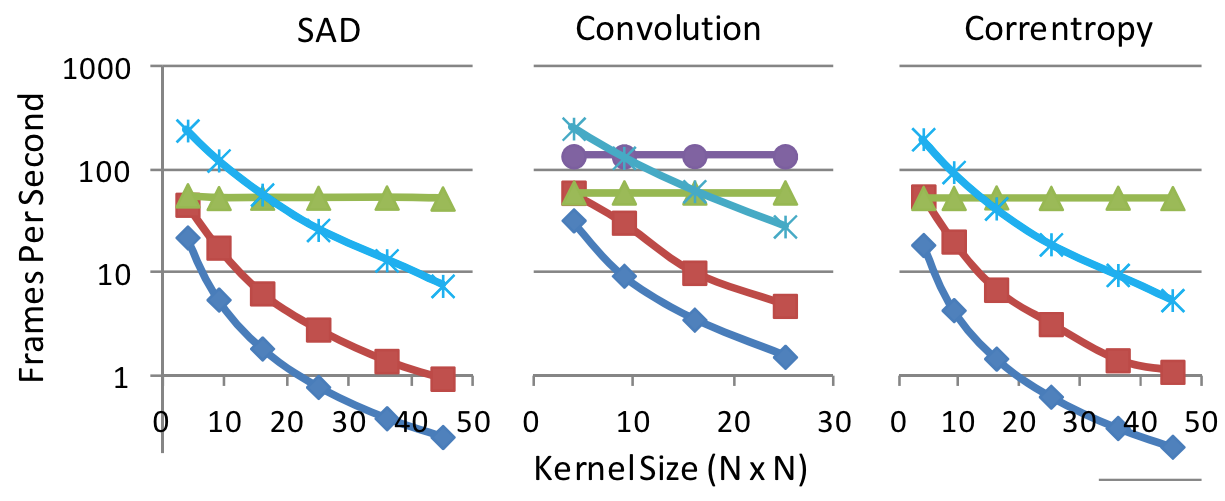
\includegraphics[width=0.7\textwidth]{./figs/cpugpufpga.png}
  \caption{Performance of all implementations in frames per 
second for SAD, 2D Convolution, and correntropy at all kernel 
sizes tested on 720p images. \cite{Fowers:2012:PEC:2145694.2145704}}
  \label{fig:cpugpufpga}
\end{figure}


The only alternative that shares all the benefits of an FPGA  based implementation would be developing an application specific integrated circuit (ASIC). An ASIC would not be easily reconfigurable but would be truly parallel in the ring network's design and could be built on the same chip as the detection hardware. The draw back of this approach however, is the enormous cost and time associated with developing an ASIC).  The design of an FPGA based system also leaves the possibility of an ASIC based implementation at a later point based on the FPGA design.
\vspace*{\fill}


 %Bg and Motiv
\chapter{Related Work}
\renewcommand{\baselinestretch}{\mystretch}
\label{chap:relwork}
%\setlength{\parindent}{0pt}


The related work can be split into 3 broad sections; DNA sequencing approachs who's implementation show interesting techniques, FPGA designs which offer insight into the design of a scalable cluster architecture and other DNA sequencers which do not provide direct algorithmic notes but instead show the current state of the art in terms of sequencing performance. All of these details will be covered below. 


\section{DNA Sequencing}

There has been a significant amount of work on computing DNA sequence correlation and DNA comparison algorithms.
In the area of DNA sequencing the majority of work has been done on software based approaches\cite{zhang2011practical}. These software solutions adopt a variety of algorithmic solutions including the Overlap-Layout-Consensus (OLC) graph based algorithm utilised here. These solutions do not provide a large amount of work on which scalable FPGA architectures can be based. This paper \cite{zhang2011practical} does however, provide a large amount of detail about existing algorithms and therefore will be useful in the evaluation stage of this project. 



There has been some significant research into parallel approaches based on CPU architectures. Despite the draw backs of parallel approaches on this architecture useful results have been found. A software algorithm called PASQUAL, implemented in C, was run on 2 Quad core Xeon processors. In this study by Lui et al \cite{liu2012pasqual}, an OLC approach is adapted in an efficient manner to run on many CPU cores, in a similar way to the approach detailed in this paper. The multiple core architecture was exploited through threading, distributing independent tasks to each core. The advantage of this technique is that no lay-off of tasks has to occur to external chips, existing tools can be used, and the data transfer times are significantly better. As a result this approach can assembles data sets of up to 6.8 billion base pairs in 15 minutes \cite{liu2012pasqual}.



In 2006, Sotiriades et al presented a DNA comparison algorithm for implementation on an FPGA\cite{sotiriades2006fpga}. The BLAST (Basic Local Alignment Search Tool) algorithm takes an input string, and compares it to a database currently stored within the processor using a process of splitting the input string into as many contiguous chunks of a fixed length as possible (allowing overlaps) and then each string is compared to the database at all points. Points where there are perfect matches are identified and the strings for these sections are extend locally in each direction in an attempt to find a longer match. The result of this algorithm is therefore a list of points where the string matches with the database.


Similar to the OLC algorithm, the advantage of this algorithm is that many strings can be compared in parallel exploiting the high data bus widths of the FPGA. Many comparisons may occur in a single clock cycle. The draw back of this approach is the high amount of memory bandwidth required to cycle through the database\cite{sotiriades2006fpga}. The limiting factor in this design therefore was the presence of RAM on the FPGA chip, this is counter to the comparison machine proposed which is limited by logic size.  This machine is more difficult to use for a real-time implementation as the database needs pre-loading, and is better suited to finding small similarities in long sequences of DNA rather than similarities through the overlap of short DNA sequences. This method is known as DNA alignment because it matches reads up against a known structure, this is distinct from the de novo sequencing discussed earlier. 


There has been a range of approaches to DNA sequencing comparison engines on FPGA. Some of the more basic applications use pre-existing processing cores, whilst the more advanced implementations focus on custom code to exploit parallelism, massively reducing computation time. 

One comparison algorithm that has been adapted for implementation on FPGA is the Smith-Waterman algorithm. Designed for comparing large databases of DNA for medical purposes the algorithm implemented by Dydal and Bala compares favourably to sequential CPU based techniques \cite{dydel2004large}. It was notable in this implementation however; that deep pipelining work was done in order to produce a design better than CPU based alternatives. Deep level pipelining has not been carried out within the provided code, this may prove necessary at a later date.


A DNA Sequence Matching Processor developed by Brown et al at California State Polytechnic University has implemented an FPGA based comparison engine \cite{brown2004dna}. This engine was limited in its algorithmic approach to the comparison problem but did address the problem of interfacing between an external FPGA and host computer. The proposed interface standard they adopted was a simple serial interface operating up to 112kbps. This design clearly showed a very low overhead such as a serial interface was still capable of operating at high enough speeds to produce a design capable of efficiently off-loading comparison work. The reason for this is the high complexity of the comparison operation in relation to the simple high-speed data interface.


As part of an investigation into using FPGAs for multi-core processing a study by Clark, Nathuji, and Lee implemented a sequencing algorithm using a MciroBlaze soft core processor \cite{clark2005using}. The Microblaze soft core processor is a Hardware Description Language based processor that can be implemented on any modern FPGA. It is a general purpose processor and can run C based code. Their attempt at parallelising the sequencing operation on this platform did not focus on speed but rather served as a proof of concept. For a data set with 1000 entries of 256 characters a processing time of 5.96 seconds was recorded. While this was not particularly fast, it showed that the comparison process scaled extremely well with an exact 4 times speed up on a 4 core processor. 



A project in 2008 by Junid et al also worked on building a custom sequencing accelerator based on the Smith-Waterman algorithm \cite{5489221}.  Their implementation used a divide and conquer technique allowing for very fast individual sequence pair comparisons with each comparison block consuming only 821 logic elements on a Altera CYCLONE II device with a delay of 10.472~ns. The system was implemented with an RS232 connection between device and computer and encoded the data in 4 bit chunks, this allowed 2 bases to be transferred to the device per control cycle. The same author then revisted this idea in 2010 with an advancement in the implementation \cite{4786759}. Through optimisations, the RS232 speed was increased by 4 times. It is important to note however, that the speed of the connection is unlikely to be the limiting factor due to the complexity of the algorithm.


As an assembler called FAssem was presented in 2013 \cite{varma2013fassem}. Based on a De Bruijn algorithm, the ``FAssem'' machine used parallel processing elements to accelerate the algorithm. As discussed earlier, the De Bruijn method is relatively memory intensive and a way in which this has been mitigated for this system is to use multiple clock domains across their device. Allowing the memory to run at significantly higher speeds (close to 300MHz). In this paper a comparison was drawn between the FPGA based implementation and a CPU based approach, the speed up achieved is shown in figure \ref{fig:fassem}. It is important to note that in this table that the processing elements (PEs) cannot be compared to the Pixels in the comparison engine algorithm introduced earlier, taking a significantly differnt structure. In terms of practical application, a total of 15 PEs could be implemented on Xilinx Virtex-6 XC6VLX130T FPGA which has 20,000 logic blocks present. This algorithm will serve as a good comparison for the algorithm presented in this report. 

\begin{figure}[h]
  \centering
  \includegraphics[width=\textwidth, page=3]{./figs/FAssem.pdf}
  \caption{Achieved Speedup with the FAssem Algorithm \cite{varma2013fassem}, PE - Processing Element}
  \label{fig:fassem}
\end{figure}




\section{FPGA Design} 


The primary research that has been examined in relation to this project is investigations and implementations of scalable FPGA clusters. As has been highlighted in the previous section the architecture of this processor has been generally fixed. The main areas of interest in scalable algorithm designs are clock synchronisation across multiple chips, inter-chip communication and bus scalability \cite{mencer2009cube}. 


Within algorithm specific processing solutions a number of methods have been explored in terms of integrating the specific processor with a host system.  These standards are shown in Figure 3 \cite{todman2005reconfigurable}  which indicates different levels to which the processor can be integrated into the system. The advantage of systems d, and e, (full integration) is the high-bandwidth between the CPU and programmable area. An example of this approach is the Altera ARM System on Chip solution; which offers a full ARM CPU core as well as a reconfigurable infrastructure on which hardware acceleration can be designed. These solutions however, are much higher cost and involve designing an entire system integrated with the application specific processor. The more common method of hardware acceleration is seen in Figure 3a, where the computer interfaces with the hardware accelerator through normal peripheral interfacing. This is the solution that would be favoured for the comparison engine as cost is an important factor in the design as well as the flexibility of being able to configure the processing unit separately to the interface with the CPU. 



A problem faced by multiple chip designs is creating an efficient way to transfer data between FPGAs. The connection of all chips to all other chips is prohibitively expensive due to the complexity of the routing as well as the physical limit of pins per chip. As a result a solution adopted by Mencer et al. was a hybrid approach of both hierarchical organisation of chips as well as a shared bus interconnect for both control and data busses \cite{mencer2009cube}. This allows an optimal level of inter-chip data throughput on the 512 chip scale that this system works on. It is important to note that within this system there is no shared memory model which simplifies the inter-connect structure. The private memory model of this system is of particular relevance to the proposed comparison engine. 
 
\begin{figure}[!h]
  \centering
  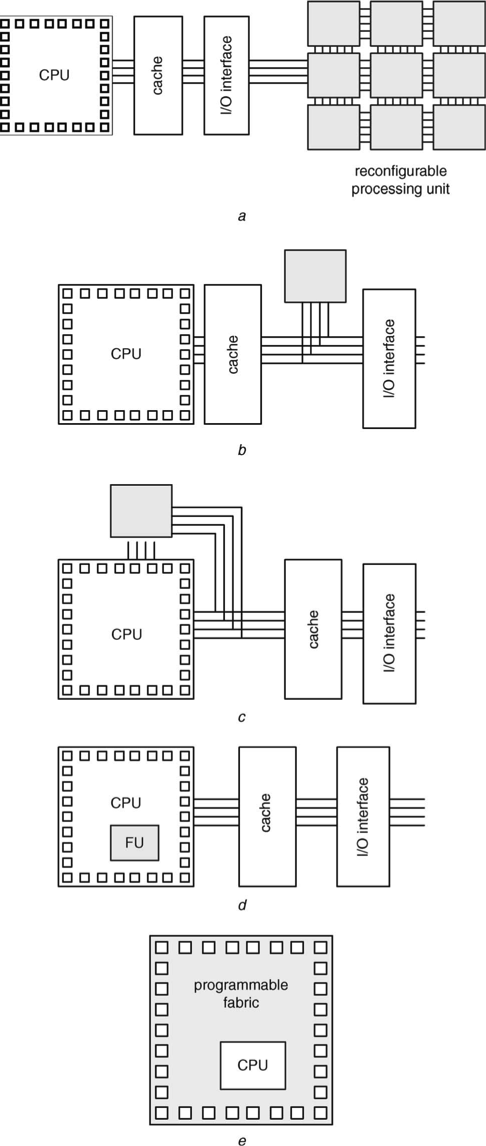
\includegraphics[width=0.5\textwidth]{./figs/fpga_cluster.png}
  \caption{Recofigurable systems; Adapted from \cite{compton2002reconfigurable}
  “(a) External stand-alone processing unit
(b) Attached processing unit
(c) Co-processor
(d) Reconfigurable functional unit
(e) Processor embedded in a reconfigurable fabric”
\cite{todman2005reconfigurable}}
  \label{fig:CE}
\end{figure}

In the design of a custom 64-FPGA cluster by Simon Moore et al. the existing PCI-Express connections present on Altera DE4 boards were converted to SATA3 connections achieving up to 6Gbps per connection between FPGAs with very low error rates (x10-15) \cite{moore2012bluehive}. This however, is a relatively high cost solution with custom board designs for the conversions and is required due to the un-structured requirement of interfacing for the neural-networking simulation. The error rate is also much higher than that required by our algorithm with simulations showing 94\% correct results even with 10\% error levels \cite{hu2012cmos}. 


The draw back of this communication structure however, was the all-to-all connection, allowing any FPGA to communicate with any other directly significantly increases the direct data throughput but has the cost of limiting the cluster to 64 chips. In this case the connections on the PCI-Express interface were at full utilisation making the cost of increasing cluster size prohibitive. One of the motivations of the DNA sequencing project is the ability to scale hardware to the required task. As a result the all-to-all approach shown here would be inappropriate. 


Another way of achieving this would be to have a common shared bus as seen in the top-level architecture of the Berkeley-Emulation-Engine (BEE2). This approach connected a 5-chip module to a 10 Gbps backbone network. This combines a hierarchical architecture with a high-speed network that also utilizes network-attached storage\cite{chang2005bee2}. The shared bus approach is an efficient solution on the assumption that board-to-board communication generally happens in random timing, if all boards were to attempt to communicate at the same time latency times would be unmanageable. In the case of this project a shared bus would be inefficient as the master FPGA receives data from the computer and then sends it out to each slave board. The result is practically all communication would ideally happen to several boards at the same time, causing latency issues. 

\section{Comparable DNA Sequencers}

As part of this project, identifying some relevant benchmarks for testing is necessary. These primarily fall into the category of CPU based algorithms as these are the simplest to implement and therefore the best to use for direct comparisons. A number of these systems exist and are available freely on the internet, a number of which have been used in sequencing tool-chains.

Velvet is a group of de novo DNA sequencing tools produced by Zerbino and Birney at the European Bioinformatics institute \cite{zerbino2008velvet}. Velvet was designed as a very short sequence assembler, using contiguous reads of around 35bp with very high coverage, this is significantly shorter than many other assemblers. This tool performs DNA assembly using a De Bruijn algorithm as well as several post-processing graph simplifications such as removing loops in the graph as well as forming blocks of reverse reads to account for reverse overlaps. This algorithm was implemented in C and during testing was run on a 64-bit linux machine. The authors conducted few tests on the algorithm, none of which discussed runtime. However the code has been made available on the European Bioinformatics webpage \cite{velvetdownload}.


The ABySS (Assembly BY Short Sequence) is a parallel tool for de novo sequencing \cite{simpson2009abyss}. The defining feature of the ABySS sequencer when it was built was that it was a truly parallel design where as sequencers such as velvet did not have the capacity. It is important to note however, with fast development in the field, systems such as Velvet have been adapted to support parallelism with tools such as OpenMPI. A common theme amongst these sequencing algorithms is that they incorporate the graph simplification and building, this is not true of the FPGA based comparison engine which makes analysis difficult. The main focus of the evaluation of ABySS in particular was the levels of correctness in the built graph, rather than the speed of the overlap comparison. This algorithm was also made available for public use on the British Columbia Genome Sciences Center (BCGSC) website \cite{ABYSSDOWNLOAD}.



A common method for sequencing short reads involves producing blocks of reads and reverse reads. This can be seen in both Velvet and tools like SSAKE, where blocks are formed of a read and its reverse. The reason for this is that the order start end of a read can not be guaranteed in the sequencing, and the algorithms commonly depend on the order of the sequence. As a result the blocking method is required so that reverse overlaps are not missed \cite{warren2007assembling}. This is commonly known as pair-end reads, as apposed to the normal single-end reads.The algorithm being implemented in this report relies exclusively on paired-end reads which are carried out automatically as part of the algorithm.



The SSAKE sequencer was implemented by Warren et al in 2006, and is also available on the BCGSC website \cite{SSAKEDOWNLOAD}. Benchmarks by the author of SSAKE achieved a 99.91\% correct sequence of the coronavirus from 476 016 reads of length 25 in a run time of 45.13 seconds on a dual core 2.2GHz AMD Opteron CPU. This will be a useful comparison to evaluate the work within this project \cite{warren2007assembling}.
\begin{figure}[h!]
\centering
  \includegraphics[width=0.65\textwidth,page=6]{./figs/comparisonlib.pdf}
  \caption{Comparison of Runtime and RAM usage for Sequencing Algorithms \cite{lin2011comparative}}
  \label{fig:comp}
\end{figure}
\pagebreak

A comparative study from the University of Shanghai for Science and Technology has produced some key comparisons between a set of sequencing algorithms. Running a variety of tests on algorithms including Velvet, ABySS, and SOAPdenovo run time and RAM usage was measured for a variety of genomes \cite{lin2011comparative}. This comparison is included in figure \ref{fig:comp}. The most important point to note from these comparisons is the long processing time required despite the hardware used. The hardware used in the test system was a cluster of 8 machines each with 2 quad-core processors. This is a highly-powerful setup and still required significant processing time for large sequence lengths. It does however, show a real application of DNA sequencer with highly relevant test data.


All the algorithms discussed in this section will be useful as comparable systems, it should be noted however that the hardware configurations used for these systems are often well beyond that used in this project. It may be necessary to factor this in when forming a comparison of these systems.







%Related Work
\chapter{Design}
\renewcommand{\baselinestretch}{\mystretch}
\label{chap:design}
\section{Overview}
The structure of this project is split into three sections; the device hardware, the device software, and host software. The device hardware is the organisation of the pre-built FPGA devices into a cluster configuration using custom inter-connectors for the cluster interface. The device software is the program that will be written onto each device and dictates their functionality. The device software comprises the bulk of the project, partitioning the computation into separate devices and handling all communication protocols between the devices. The host software runs on a host machine connected to the cluster and provides all source data for the system as well as receiving all the output data from the cluster system.


In this project the available hardware has been the motivating design limitation, and so discussion of the hardware configuration is discussed first, the characteristics of which will motivate the design decisions made in the rest of the design.

%\setlength{\parindent}{0pt}
\section{Hardware}
The motivation of this project was a scalable system and the design of the HDL is intended to be built such that it can be implemented on any FPGA hardware with the relevant ports. For the purposes of testing in this project three DE0 FPGAs will be used (shown in Figure \ref{fig:de0}).


The Terasic DE0 board contains an Altera CYCLONE III FPGA with 15,408 logic elements and 512kb of memory. This chip is capable of hosting around 9 pixels from the original algorithm within around 10 000 logic elements. This board has a relatively large number of general purpose input/output ports with 2 40-pin connectors on the side of the board. It also has a 5-pin RS232 specification UART which may be used for host computer to device simulation. 

In order to  ensure that the design of the system is scalable to other architectures and interfaces, the UART controller can be logically partitioned and replaced in other applications as will be discussed in the HDL design.  First estimates of the number of interconnect ports needed are around 40 pins minimum with the scaling as the design parameters change. As these FPGA development boards are available freely within the department they will be used for the prototype system design. It is important to note however, that this should not impact the design in such a way that stops the design from being easily moved to other boards when necessary. A secondary benefit of this board is the large number of user input/output ports such as 4 7-segment displays which can be used for debugging and progress checking.  This board was freely available within the department and therefore made a good low cost prototyping unit, however these boards can be bought at a retail price of \$120. 


\begin{figure}[h!]
  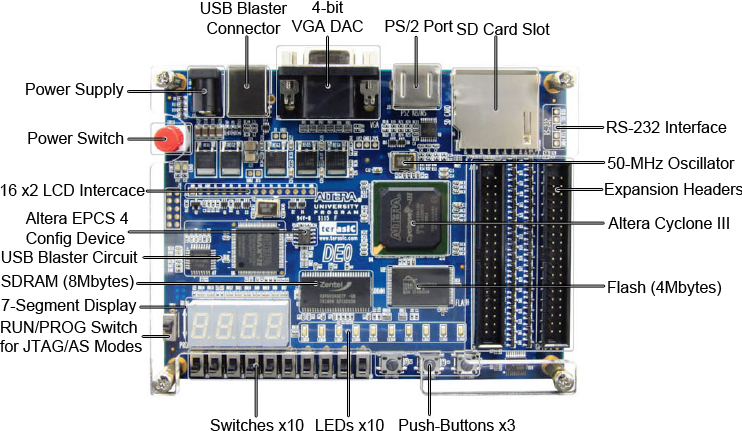
\includegraphics[width=\textwidth]{./figs/de0.png}
  \caption{Terasic DE0 FPGA Board}
  \label{fig:de0}
\end{figure}


An important decision to be made in the design of the hardware was whether to use a common clock across all the devices, or to use separate clocking. The advantage of the single clock is that the processors can work in lock-step reducing communication delays and simplifying the interconnect protocol. However, a common clock places other limitations on the design. The common clock design limits the clock frequency of all the devices to the speed at which the inter-FPGA communication can happen, this may lower the theoretical maximum clock speed, however the design already runs at a relatively low clock speed and the intentional is to overcome this limitation with parallelisation. The common clock will need to be considered in the testing stage, as identifying the clock speed where correct operation is primarily done through trial and error with a trade-off between bit-error rates and speed. The ring network design of this system favours the common clock approach as all communication is exclusively done with nearest neighbours, limiting the length of the inter-FPGA communications. 

\subsubsection{Inter-Device Communication Hardware}
All inter-FPGA communications will be done using the 40-pin GPIO connectors that were discussed earlier. The communication is done exclusively in a ring, which lends itself to a dual connector geometry. For each device the second GPIO connector will be linked to the first GPIO connector of the next device, with the final device looping back to the first connector of the first device. This is better than all-to-all communication, as that would scale extremely badly with number of devices as well as using far more ports. This takes care of the communication, however it is also necessary to have a shared global clock. This is achieved by separating one of the wires from the ribbon cable that connects the GPIO and connecting it together. This design is shown in figure \ref{fig:interfpga}, and is shown implemented on the board in the implementation section, figure \ref{fig:cluster}. The practical applications of this is also considered in the implementation section where the speed of the connection is analysed. 

\begin{figure}[h!]
  \includegraphics[width=\textwidth]{./figs/interfpga.pdf}
  \caption{Inter-FPGA Communication Hardware Setup}
  \label{fig:interfpga}
\end{figure}

\subsubsection{UART Hardware}
The UART interface on the board is theoretically designed to interface with any other RS232 standard UART controller, and the data streaming protocol will be covered in the Device Software section. For the purposes of interfacing with a host computer a USB to UART cable has been bought. Capable of up to 1~Mbaud the FTDI USB-RS232, this cable allows communication between the host software and device software using a virtual COM port for which there are multiple Application Programming Interfaces (APIs) available. The 1~MBaud limit allows up to 921,600 bits per second to be transmitted, when this is considered in the scope of the streaming project where each pixel has  a 2 bit data sample taken in the order of seconds and a DE0 FPGA can fit around 10 Pixels per device, the data rates this interface is capable of far exceed the rates needed. Only when devices with hundreds of pixels are present or extremely large arrays of devices are used will this present a problem. On the DE0 board a level shifter is present, this turns the 3.3v device signals into the $\pm$13v standard that RS232 uses.
 %hardware
\section{Device Software}




\subsection{Overview}

The device software makes up the bulk of the work done within this project. The basic algorithm devised by Y Hu et al is mostly unmodified, with the modifications limited primarily to the communication of data between devices. This work can broadly be split into three sections; the data input handler, the inter-FPGA communication, and the library data read-out. The data input handler interfaces with the host software and distributes the input data across the system. The inter-FPGA communication controls the algorithm's execution to guarantee synchronisation across the multiple devices. The result data handler returns the overlap libraries produced by each pixel via the UART interface with the host. In order to explain the design of these three sub-systems it is important to understand the over-arching aims of the device software. The top level of this system can be seen in figure  \ref{fig:tld}. Each device contains a data Input/Output (IO) handler as well as small modifications to the global controller. Through maintaining the same structure as far as possible, the implementation minimises the impact of cross-device interfacing on each device's operations.

What this approach does in terms of the algorithm is split work in a uniform fashion, increasing the work done by a single pixel, but keeping the total work done per FPGA the same. This can be explained by viewing an all-against-all comparison as a matrix of comparisons.




$
\text{Comparison Matrix} =  
\begin{pmatrix}
  F(a_{1},a_{1}) & F(a_{1},a_{2})  & \cdots & F(a_{1},a_{n}) \\
  F(a_{2},a_{1}) & F(a_{2},a_{2})  & \cdots & F(a_{2},a_{n}) \\
  \vdots  & \vdots   & \ddots & \vdots   \\
  F(a_{n},a_{1}) & F(a_{n},a_{2}) & \cdots & F(a_{n},a_{n}) \\
 \end{pmatrix}  
 $
 
 
Within this matrix each pixel does one column of work, performing the comparison between 1 common sequence and all other sequences. However, there are no true dependencies within this matrix, any comparison can be carried out in any order. In the original comparison engine, the movement of data around the chip was the driving factor, so each pixel started with it's own sequence, and then used data forwarded around the ring network. This can be understood within the matrix as each pixel starting on it's entry in the leading diagonal of the matrix and then working up the matrix, looping at the top down to the bottom. In this way all the comparisons happen together in lockstep.

Splitting this algorithm across mutliple devices is complex due to this fact however, as currently pixels only do the same number of comparisons as there are on the board. In the newer design one of these pixels will still do the comparisons with all the sequences from the entire cluster, and as such the link between number of pixels present and  number of comparison cycles must be broken. Each device can then be viewed as a rectangular matrix, which when concatenated form the previous complete matrix as shown below for 3 devices.




\begin{align*}
\text{FPGA}_0
 &=
 \begin{pmatrix}
  F(a_{1},a_{1}) & F(a_{1},a_{2})  & \cdots & F(a_{1},a_{\frac{n}{3} }) \\
  F(a_{2},a_{1}) & F(a_{2},a_{2})  & \cdots & F(a_{2},a_{\frac{n}{3} }) \\
  \vdots  & \vdots & \ddots & \vdots   \\
  F(a_{n},a_{1}) & F(a_{n},a_{2})  & \cdots & F(a_{n},a_{\frac{n}{3} }) \\
 \end{pmatrix} \\
\text{FPGA}_1
 &=
 \begin{pmatrix}
  F(a_{1},a_{\frac{n}{3}+1}) & F(a_{1},a_{\frac{n}{3}+2})  & \cdots & F(a_{1},a_{\frac{2n}{3}}) \\
  F(a_{2},a_{\frac{n}{3}+1}) & F(a_{2},a_{\frac{n}{3}+2})  & \cdots & F(a_{2},a_{\frac{2n}{3}}) \\
  \vdots  & \vdots & \ddots & \vdots   \\
  F(a_{2n},a_{\frac{n}{3}+1}) & F(a_{n},a_{\frac{n}{3}+2})  & \cdots & F(a_{n},a_{\frac{2n}{3}})
 \end{pmatrix} \\
 \text{FPGA}_2
 &=
 \begin{pmatrix}
  F(a_{1},a_{\frac{2n}{3}+1}) & F(a_{1},a_{\frac{2n}{3}+2})  & \cdots & F(a_{1},a_{n}) \\
  F(a_{2},a_{\frac{2n}{3}+1}) & F(a_{2},a_{\frac{2n}{3}+2})  & \cdots & F(a_{2},a_{n}) \\
  \vdots  & \vdots & \ddots & \vdots   \\
  F(a_{2n},a_{\frac{2n}{3}+1}) & F(a_{n},a_{\frac{2n}{3}+2})  & \cdots & F(a_{n},a_{n})
 \end{pmatrix} \\
 \\
\text{Comparison Matrix} &= \text{FPGA}_0 \parallel \text{FPGA}_1 \parallel \text{FPGA}_2 \\
\end{align*} 


This shows there are now $\frac{n}{y}$ pixels per device with y devices, but each pixel still does n comparisons. This idea will be revisited later in discussions of other future work.
 
The decision was made to favour a shared clock, lockstep operation design for this implementation, the reason for this is that the ring network design has a natural dependancy loop. This would mean any discrepancy in throughput would cause the system to  hang both for the slowest element of the system but also for communication within the system and would require significant local data storage to mitigate local sources of latency such as long memory accesses on a single FPGA. The lock step design introduces a problem of both guaranteeing coherence across the system as well as practical limitations on clock speed. These practical limitations will be discussed in the implementation section.



The algorithm provided gives a number of important features that must be kept, stream processing and independent logical elements being the most important. 
\begin{sidewaysfigure}[p]
  \centering
  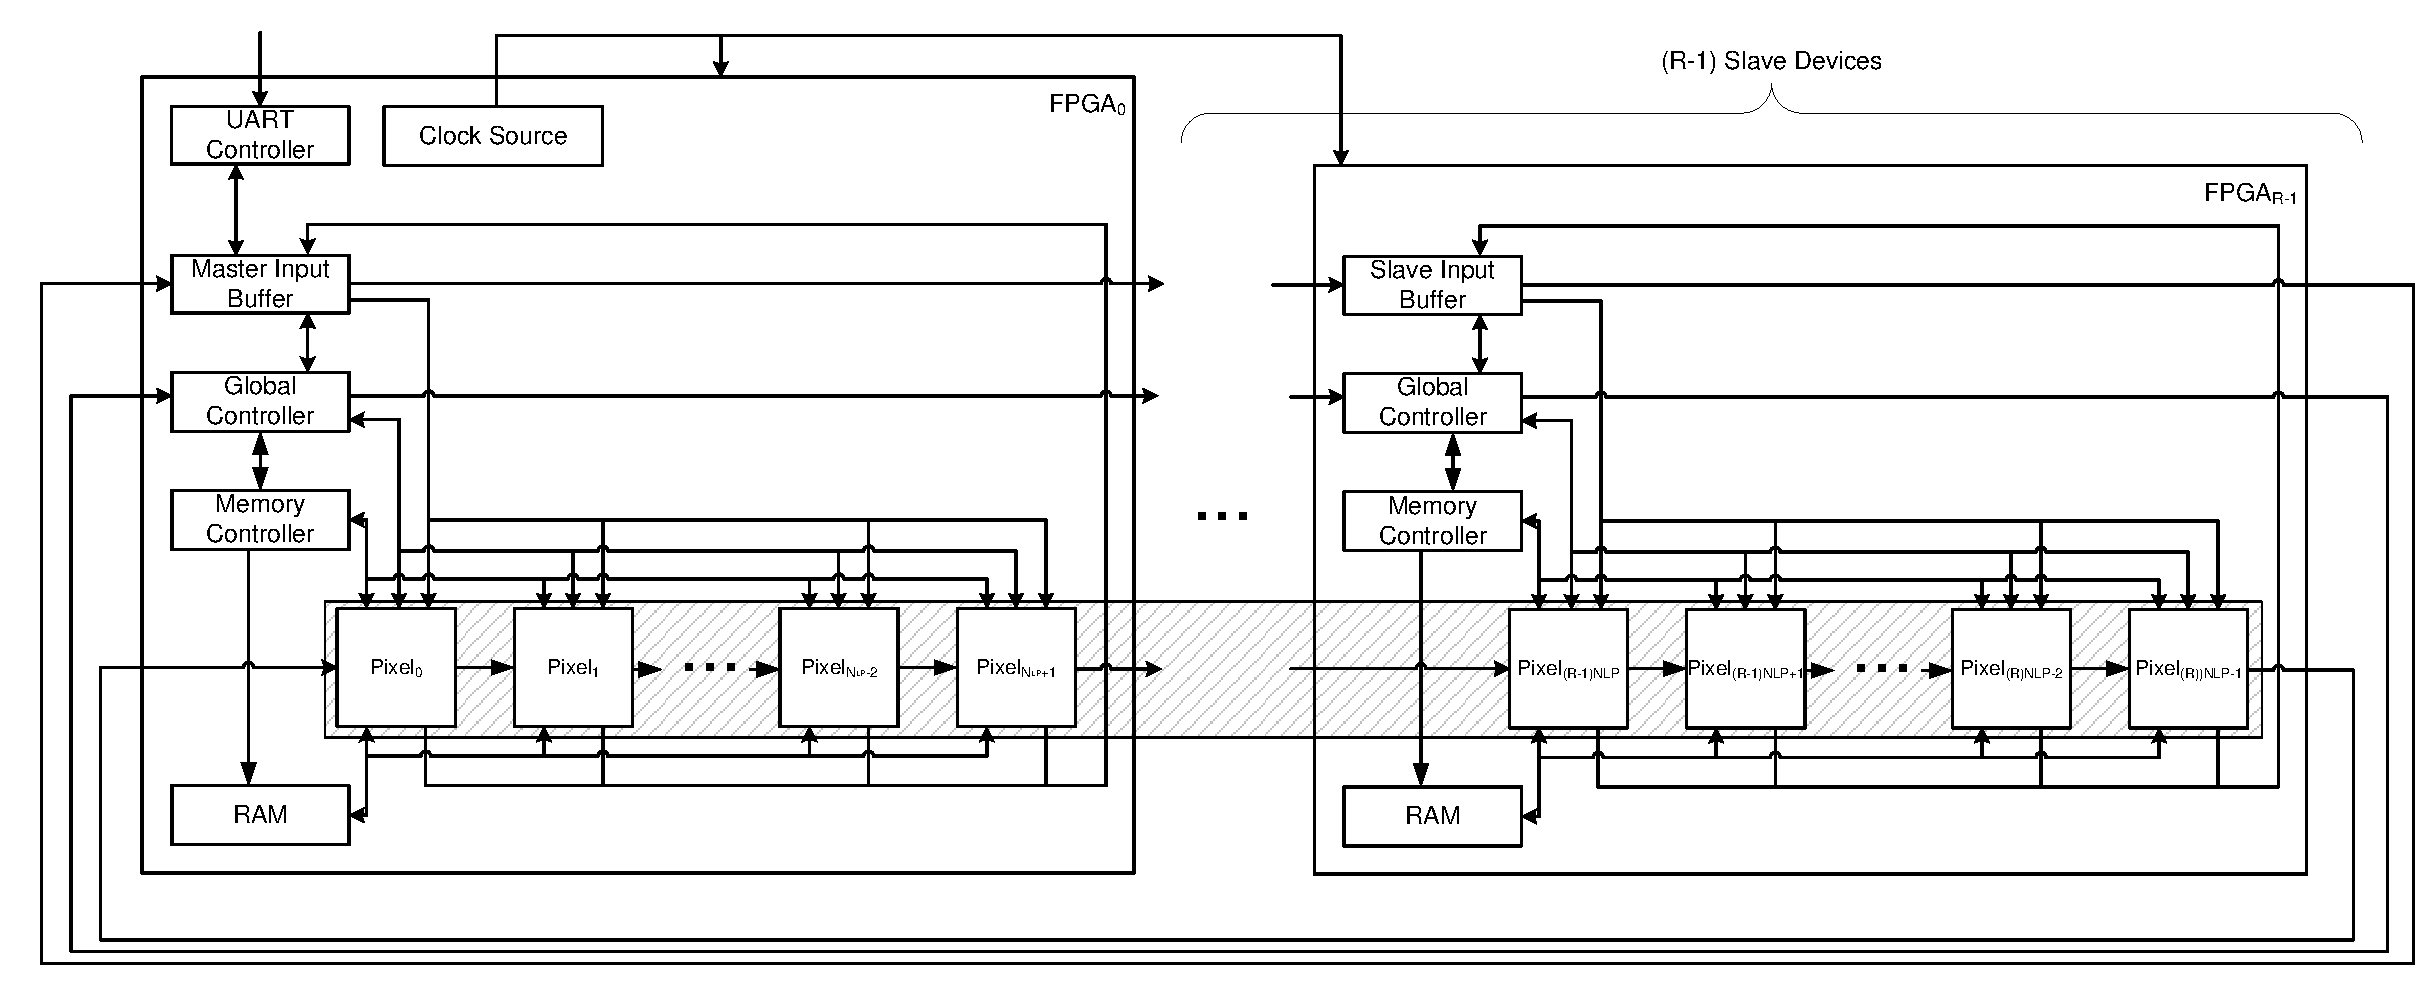
\includegraphics[width=\textheight]{./figs/MFPGA.pdf}
  \caption{Top Level Diagram, 1 Host, R-1 Slave Devices}
  \label{fig:tld}
\end{sidewaysfigure}


\subsection{Data Input Handler}
All the data transfers with the host machine are done via one connection, this is present only on a master FPGA, the other devices received data forwarded around the ring network. It is important however, that the processing happens in lock step, as a result the input data must be available on all FPGAs at the same time. This can be done either through communication between FPGAs or through strict control of the data path. As communication is relatively expensive (due to the high latency of sending signals around the ring network) a fixed latency approach has been chosen. As an over-arching design decision, all signals sent between devices are clocked out and in with no logic. This guarantees the maximum allowance for the data path between devices. 

\subsubsection{The Master UART Connection}
Present only on the master device, the UART interface works at the $\pm$13~volt RS232 specification with the data transfer protocol shown in figure \ref{fig:UART}. The UART controls both the incoming data to be processed and the outgoing data reported to the host. The format of the incoming data is a stream ordered first by read order then by pixel order. The data rate achieved by this interface is up to 1~Mbaud, this is 1 million symbols per second. In the context of  a device that can fit up to 100 pixels as discussed in the complexity analysis of the algorithm, this is significantly faster than necessary. The primary goals of the UART connection is fast enough data rates with low error rates. This is achieved with the oversampled interface. This means for a 1~MBaud system running on  a device with a faster clock, each data bit is sampled multiple times, thus reducing error rates. 
\begin{figure}[!h]
  \centering
  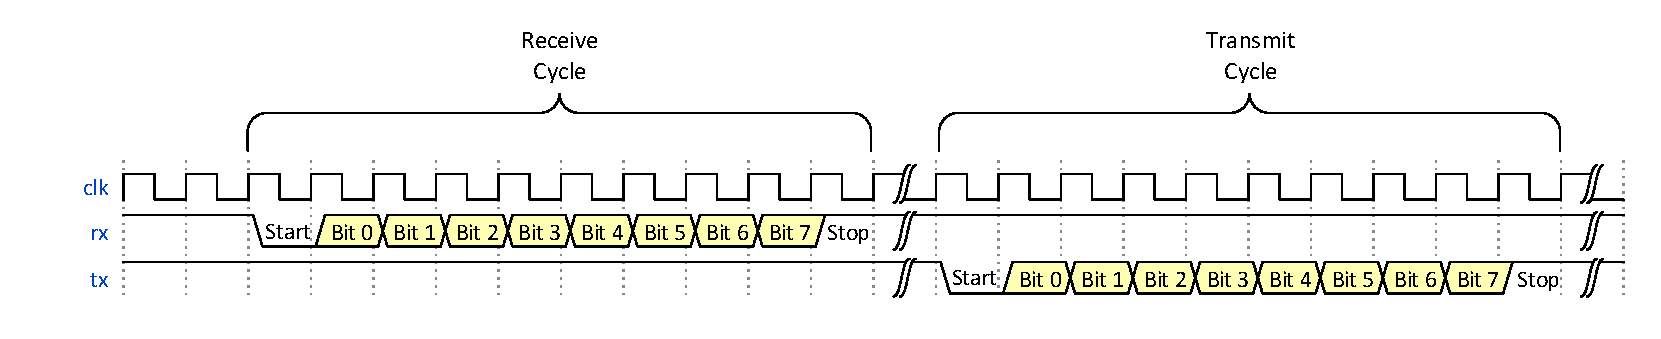
\includegraphics[width=\textwidth]{./figs/UART.pdf}
  \caption{UART Interface Protocol}
  \label{fig:UART}
\end{figure}


The UART controller on the device is designed as a separate module with a simple interface. The reason for this is that if necessary, different external interfaces can replace the UART if necessary. This would be common when implementing the design different hardware which may only have connections for protocols like USB or PCI-Express. In the case of this project an external piece of code was used to interface with the UART standard, this was done as UART interfaces are a standard piece of code and there is little value in reproducing this work.


\subsubsection{Distribution of Input Data}
\begin{figure}[!h]
  \centering
  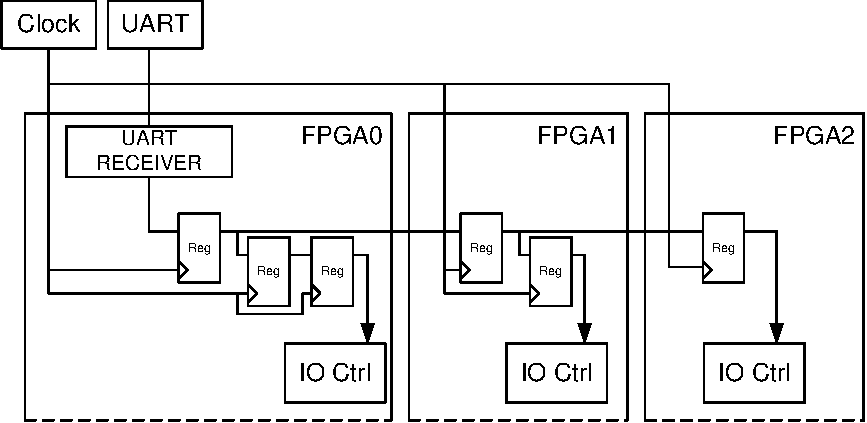
\includegraphics[width=0.8\textwidth]{./figs/input_delay.pdf}
  \caption{Input Delay System Example for 3 Devices}
  \label{fig:delay}
\end{figure}
One of the keys to the lock-step design is ensuring that all the input data appears available to the processor across all devices at the same time. This can be ensured by a simple system of delay registers. This system is shown in figure \ref{fig:delay}, it ensures that all FPGA input adaptors receives the data in lock step. Technically this requires the forwarding of more data than necessary, as data for all pixels reach all FPGAs, as well as invalid data being forwarded with an invalid flag. However, removing this redundancy could not shorten the delay and complicates the logic so it was decided to be preferable to complex logic. The output of this delay cycle is identical across all devices, an 8 bit data chunk with a valid signal going in to the data format translator. The result of this process is a latency of N cycles, where N is the number of devices in the cluster. It is important to note that latency is not an issue in terms of the end speed of the cluster, as it will be hidden during the processing time and is relatively negligible. 






\subsubsection{Data Format Translation}
As discussed earlier, the UART used to input data (and the interface to forward the data between FPGAs) consists of a byte based transmission system. This means data comes in 4 pixels at a time, however the system requires 2 bits to be sent to each pixel in parallel. This requires a complex data width adaptation. This is achieved by clocking data into a wide register 8 bits at a time, and then writing it out to a First In First Out (FIFO) memory structure at the correct bit width. The memory structure adds a small amount of processing flexibility in the case that data is coming in faster than can be processed. In this project the FIFO can store all input data, this is possible due to the fact the comparison engine is very logic element intensive but not memory intensive. A correctly designed FIFO maps to a memory bits on chip, a separate resource to the logic utilisation. As discussed earlier, for a 9 pixel design over 80\% of the logic elements are used on a DE0 device, but less than 1\% of the memory is used. The translation system is a relatively complex translation as is shown in figure \ref{fig:translator}. It is important to note that this width adaptor requires more than 1 pixel per device, otherwise the input adaptor register will be overwritten by a single input twice in a single cycle.

\begin{figure}[!h]
  \centering
  \includegraphics[width=0.9\textwidth]{./figs/input_adaptor.pdf}
  \caption{Input Adaptor, N$_{LP}$-Number of Local Pixels, N$_{TP}$-Number of Total Pixels}
  \label{fig:translator}
\end{figure}



\subsection{Inter-FPGA Communication}

Inter-FPGA communication provides both algorithm synchronisation and extension of the ring network. As shown in figure \ref{fig:tld} the global controller on each device communicates and the ring network communicates.

The extension of the ring network is the most simple, the communication that would normally happen forwarding suffix data between pixels is routed across the GPIO ports as described in the hardware section. Algorithmically this is identical to the original implementation but limits the clock speed due to data transfer rates. This interface is an important limiting factor for the design. The number of connectors between the devices for the ring network is 4 bits for every parallel string being forwarded, this quickly reaches the limits of the number of connectors available. 


The global controller interface is more complex due to the non-fixed nature of the state machine. The state machine for the original algorithm is shown in figure \ref{fig:ctrlfsm}. It can be seen, the only conditional transitions are on input data being available, and checking for pixels to complete. The other transitions are all determined by fixed length states. 


\begin{figure}[!h]
  \centering
  \includegraphics[width=\textwidth]{./figs/ctrl_fsm.pdf}
  \caption{Algorithm Global Controller Finite State Machine}
  \label{fig:ctrlfsm}
\end{figure}


The transition for moving into the read state is conditional on the data being available, as is covered in the previous section, measures have been taken to ensure this happens identically on all devices. The transition from the Wait for All state to Idle state is more difficult however. All pixels must report ready to the controller before the state can proceed. This is very difficult to do across several FPGAs fast, so instead a distributed mechanism has been designed. Each device has all it's pixels report, when all pixels on the master report  it forwards a done signal. Each slave then forwards this signal only when its own pixels are done. When the master receives the done signal back, it then sends a proceed signal and waits a fixed length of time, each slave forwards this signal immediately and waits for 1 fewer cycles. In this way it is guaranteed they count down together. Finally at the end of the countdown they proceed to the next step.

The net result of this in terms of cycles per comparison is that one cycle through the state machine (which corresponds to 1 new piece of data) is increased by $2 \times $the number of pixels. This protocol lowers the speed of comparisons in cycle count, but allows for the fast shared clock. The impact of this will be studied in the testing and evaluation sections. 





\subsection{Result Data Handler}

The result data in the algorithm is stored on a per pixel basis in a library of complex data structures. This library is shown in the listing below. These library entries are known as overlap seeds.


 \begin{center}

 \begin{minipage}{\textwidth}
\lstset{language=python, numbers=left, showspaces=false,
    showstringspaces=false, tabsize=4, breaklines=true, captionpos=b, numbersep=5pt }
\begin{lstlisting}[frame=single,caption=Result Data Format, label=listing:record]
	TYPE SEED IS RECORD
		posi   : RD_INT_TYPE; -- range 0 to READ_LENGTH
		rota   : PIXEL_INT_TYPE; --range 0 to PIXEL_COUNT
		score  : EDDI_INT_TYPE; -- range 0 to REDUNDANCY + 1
		chk_wt : WAIT_INT_TYPE; -- range 0 to INFIX_LENGTH
		bases  : BASE_VECT; -- array 0 to 2 REDUNDANCY + 1
		lock   : STD_LOGIC; 
	END RECORD;
\end{lstlisting}
 \end{minipage}
\end{center}
This data structure is highly dependant on the parameters of the comparison engine and therefore the size is variable. Each library has a parameterisable number of entries and there is one library per pixel. To write this data out across the UART 3 processes must take place. First the data must be gathered per deice and formatted for transfer, then the data must be gathered on the master device, finally the data must be sent out across the UART.
\begin{figure}[!h]
  \centering
  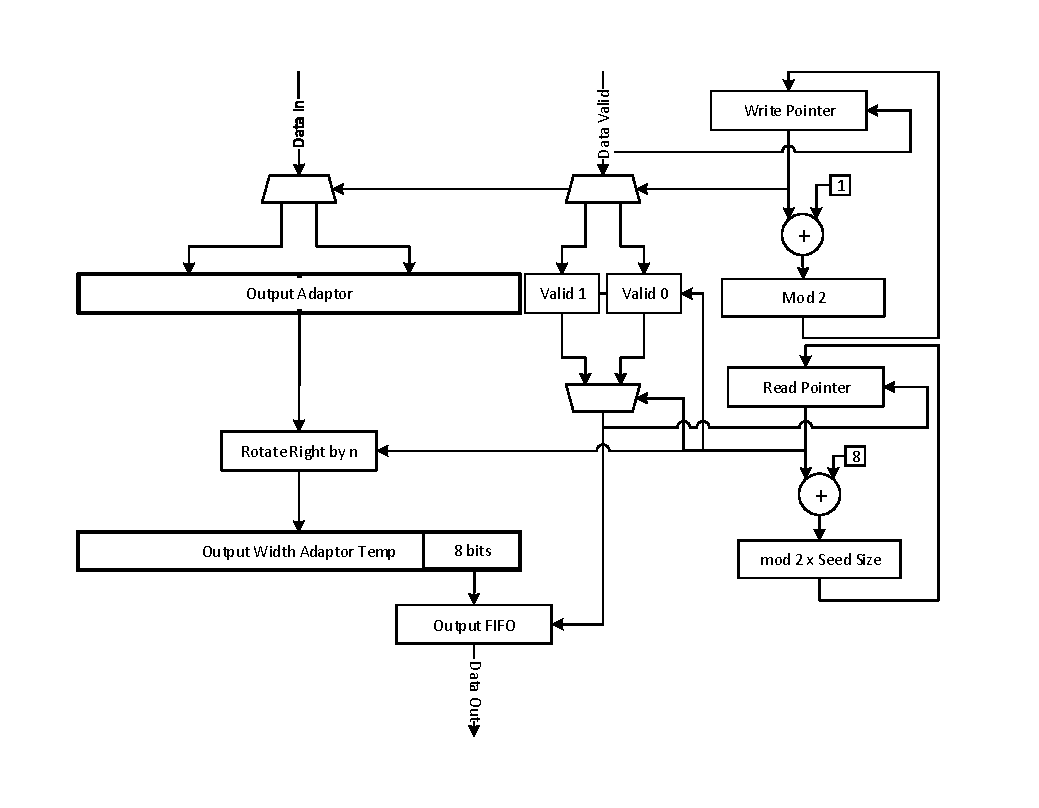
\includegraphics[width=\textwidth]{./figs/output_adaptor.pdf}
  \caption{Output Width Adaptor}
  \label{fig:owa}
\end{figure}

The first stage requires the record to be flattened into a single vector data type. The IO controller on each device then cycles through each pixel requesting their records until they report the end. This then creates a local copy of the libraries together, however this is formed of very large data types that are not suitable for transferring off-chip. Another data width adaptation is required to allow communication between devices, shown in figure \ref{fig:owa}. 


Having translated the current library data into a transferrable format this has to transferred across the ring network. Inter-FPGA communication is already quite high, requiring a large amount of connections so it is best to re-use the data forwarding connections that were used for the input data. The time multiplexing of this connection can safely be used with no effect on performance. The data on the ring network must be transferred in a fixed order to allow reconstruction of the library on the host, this is done by transferring all data from the first slave, followed by an end signal. Each slave in the network forwards the data and uses the stop signal as a prompt to append their own data. The master FPGA caches this data and transmits it over UART, appending it's own library. The impact of caching the full library on one device is small. As covered earlier, memory usage is already extremely low and the library data by nature is only a small fraction of the input data.



 %software
\section{Host Software}
One of the stated goals of this project was to produce a real-time system and a suggested way to achieve this was through the use of a streaming interface between the DNA detection hardware and assembly algorithm. Compatability with this goal is covered in the device software section of the report covering the UART streaming interface. However, for the purposes of this report and for testing and verification of the project the host software built here will use a fixed data source with generated test data. 

In order to simplify the host side interface with the device software an FTDI cable was used (as covered in the Device Hardware section). The host software has two simple functions, to read data from a text file and transmit it to the UART, and read result data from the UART out to another text file. In order to maximise backwards compatibility and ease of testing, I will adopt the formatting of the input data used by Y Hu in his test bench for the original algorithm. This consists of N lines of M length, where N is the number of pixels and M is the read length, the DNA bases are represented by capital letters; A- Adenine, T- Thymine, C- Cytosine and G- Guanine. An example input file is shown in \ref{listing:example}. This format is a standard format used in a number of tools including the ABySS sequencer and the BLAST sequencer \cite{ABySS}\cite{BLAST}. \\


\begin{minipage}{0.8\textwidth}

\begin{center}

 \lstset{numbers=left, showspaces=false, showstringspaces=false, tabsize=4, basicstyle=\tt, breaklines=true, captionpos=b, numbersep=5pt }
\begin{lstlisting}[ frame=single,caption=Input Data Format Example; 9 Pixels\, Read length 50, label=listing:example]
 CGAGGGATGTCTCTTGCGTGTCAAACAACTCTCTTTCGTTACTATGCGGG
 AATTCGTATCAACATATGTCGGGGTTCATATGGACACTATAGGCAGGTGT
 AGATAGCCGTTTCGAAGTTGAATGACTGTGCCCAGAACGTACTCAGATCC
 AGACAGCATCAAAGCACACTATTCCCGACCGTAGGGACCTAACGGATTAG
 ATCGTAGAACCCGAAGACGGAGTTCCCGTAATAGAGCCAAAGTATGTTGT
 ACACGTGTCTAGCACGGCAAACGGGCCAGGGTCCCTATGGGTAAGGACCG
 GTCATGCGCCCGTTGAAGGCTTAGTCTAAATTGTATTTAGCACCATGGCT
 GGATTAAATGCGCATGCAACGGATACTGAACATGGGCAATACGCGTTAAC
 GACCCGAAGGTTTTCGGCTGCGACTCCAACGACCGTCTGTAGGCTGGATT
\end{lstlisting}

\end{center}
\end{minipage}

In order to make this compatible with the streaming interface, this input data must then be converted to binary and re-ordered. The binary translation for each base is as follows: A: 00, T: 01, C: 10, G:11. The streaming interface requires that the data is transferred ordered first by read number, then by pixel count. This translation is done by the code listed in Appendix \ref{App:Host_Software}

Similarly the host software is required to unpack the output data from the FPGA, this is also done through simple python bit manipulation and writes the output to a file, ordering the library data in the same format as it is present on the FPGA local memory. This can then be used to carry out a comparison with the simulated data in the test bench setting or used to recombine the data in a true application of the algorithm. 

This functionality is achieved through a python script that can be run from the command-line, passing in the parameters dictating read length, pixel count and the location of the source data. This script automatically interfaces with the device and prints the result data to a timestamped text file in the destination directory. This code is included in appendix \ref{App:Host_Software} and a guide how to use this is included in the user guide appendix \ref{App:UserGuide}.
\vspace*{\fill} %Host Software %Design
\chapter{Implementation}
\renewcommand{\baselinestretch}{\mystretch}
\label{chap:implementation}

\begin{figure}[h!]
  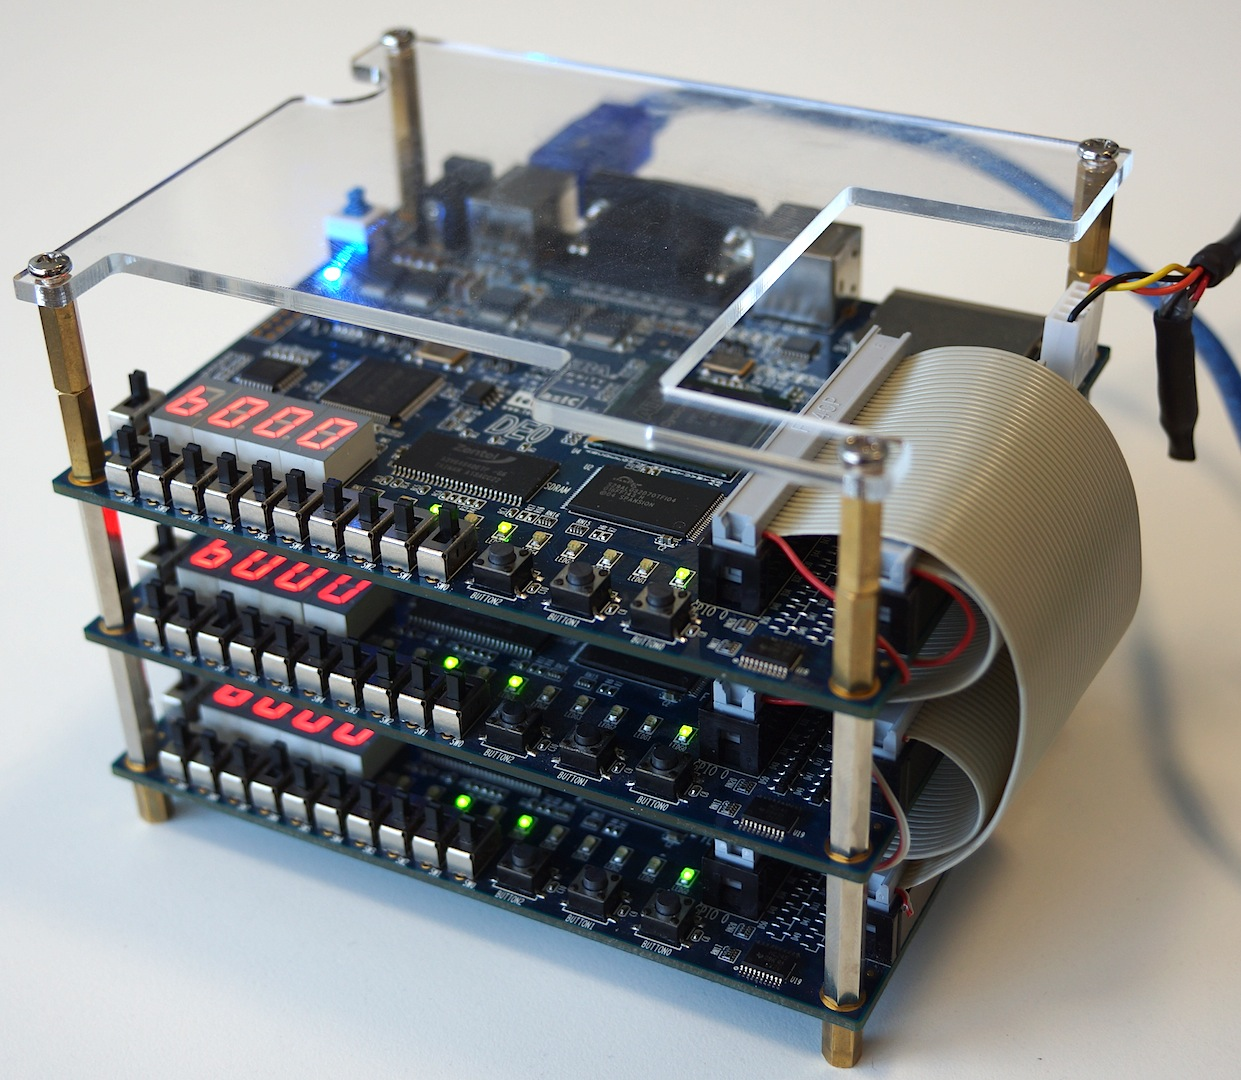
\includegraphics[width=\textwidth]{./figs/cluster.jpg}
  \caption{Hardware Implementation}
  \label{fig:cluster}
\end{figure}
%\setlength{\parindent}{0pt}
As discussed in the design section, one of the main features of this design was organising the processors to run in lockstep. This meant there were no internal data transfer protocols other than simple ready/available data signals. As a result the vast majority of the design translated from simulation to device implementation in a straight forward way. The only non-deterministic element of the design was the shared clock across multiple devices, this element required some simple analysis to identify the limits. The clock frequency needs fine control in order to limit the error rates in the data transfer. This was done by using a phase locked loop (PLL) on the master device, this takes the local 50~MHz clock as an input and outputs a compile time set frequency. This clock is then put out across 1 GPIO pin. As described in the design section this is then used as the clock input of all the devices. 

The clock frequency maximum set by the on board logic was 31MHz, ideally the inter-FPGA communication also fits this limit, allowing maximum speed of operation. The velocity of propagation for the ribbon cable is 4.53~nsM${^{-1}}$ \cite{ribbon}. Assuming a total cable length of 15cm, including the propagation from chip to connector (it is safe to assume the PCB is a better propagator than the cable), the total latency of a signal is 
\begin{align*}
\text{Propagation Delay} &= \text{Propagation Velocity} \times \text{distance} \\
&= 4.53 \times 0.15 \\ 
&= 0.6795~\text{ns} \\
\text{Fmax} &= \frac{1}{\text{Propagation Delay} + \text{Input Delay} + \text{Output Delay}} \\
\text{Fmax} &\approx  \frac{1}{0.680 \times 10^{-9} + 2.19 \times 10^{-9} + 0.915 \times 10^{-9}} \\
\vspace{5em}
&= 260~\text{MHz}
\end{align*}

These calculations use IO delay characteristics as detailed in the Altera CYCLONE III datasheet \cite{altcyc}.

As can be seen from these estimations, as long as the inputs and outputs are registered, there should be enough slack to run the processor at the limit the pixels will allow. It is important having made these estimations to test these in a practical setting.


Another implementation problem to consider is the clock skew. The clock can take a variable amount of time to travel both across chip and between chips. This is easy to model within a single device, using the toolchains provided by FPGA manufacturers. However, across chips there are no modelling tools. In a similar way to the Fmax calculation, the clock skew will be effected by the number of devices and their distance apart. However, it is possible to try and control the clock skew by ensuring that the clock source is connected to all the devices in a similar fashion. On the DE0 FPGA this has been achieved by sending the clock out of the master device and then splitting the signal from a shared point to go to each device with an identical connection. This still requires testing in a practical environment however. For larger clusters of FPGAs on more expensive technologies there are different systems that can be used. The ribbon cable that is used in this implementation isn't a particularly high quality transmitter for this purpose, other devices have serial digital interfaces which may be used for clock sharing, this provide much higher quality channels across which the clock can be shared.


There are also steps that can be taken within the compilation of the HDL for each device. Using Altera's TimeQuest timing analyser priorities can be set during compilation to guarantee certain routing limits. For this project the device IO is important as this is where bit-errors are likely to occur and can affect maximum frequency for the cluster. As part of the compilation process these paths have had delays set so that the router adjusts for the fact that signals coming from these paths have been slightly delayed as covered by the calculations earlier. TimeQuest also indicates paths that are likely to fail the requirements of timing, in the case of this project some modifications were made to the width adaptor so that logic was minimised between clock cycles. One particular issue arose that caused bad performance was using an integer to point to where data needed to go. This integer by default compiles to a 32 bit signal which causes an extremely large amount of logic as it was involved in both logical shifts as well as conditional clauses, by adding a range to this integer the size of the vector was cut down. This massively increased on chip performance. In one test case this lowered the logic on a device by 20,000 logic elements.

\subsection{Error Tolerance}

An important part of the practical implementation is error rates due to inter-device communication, however this can be mitigated to some extent. The comparison engine that was adopted for implementation has a limited level of error tolerance \cite{hu2012cmos}. In figure \ref{fig:err} the levels at which errors can be tolerated are shown, with similarity to the correct sequence shown with given sub-sequence error rates. This tolerance means that even operation where bit-wise correct operation is unachievable valuable results can be calculated.

\begin{figure}[h!]
\centering
  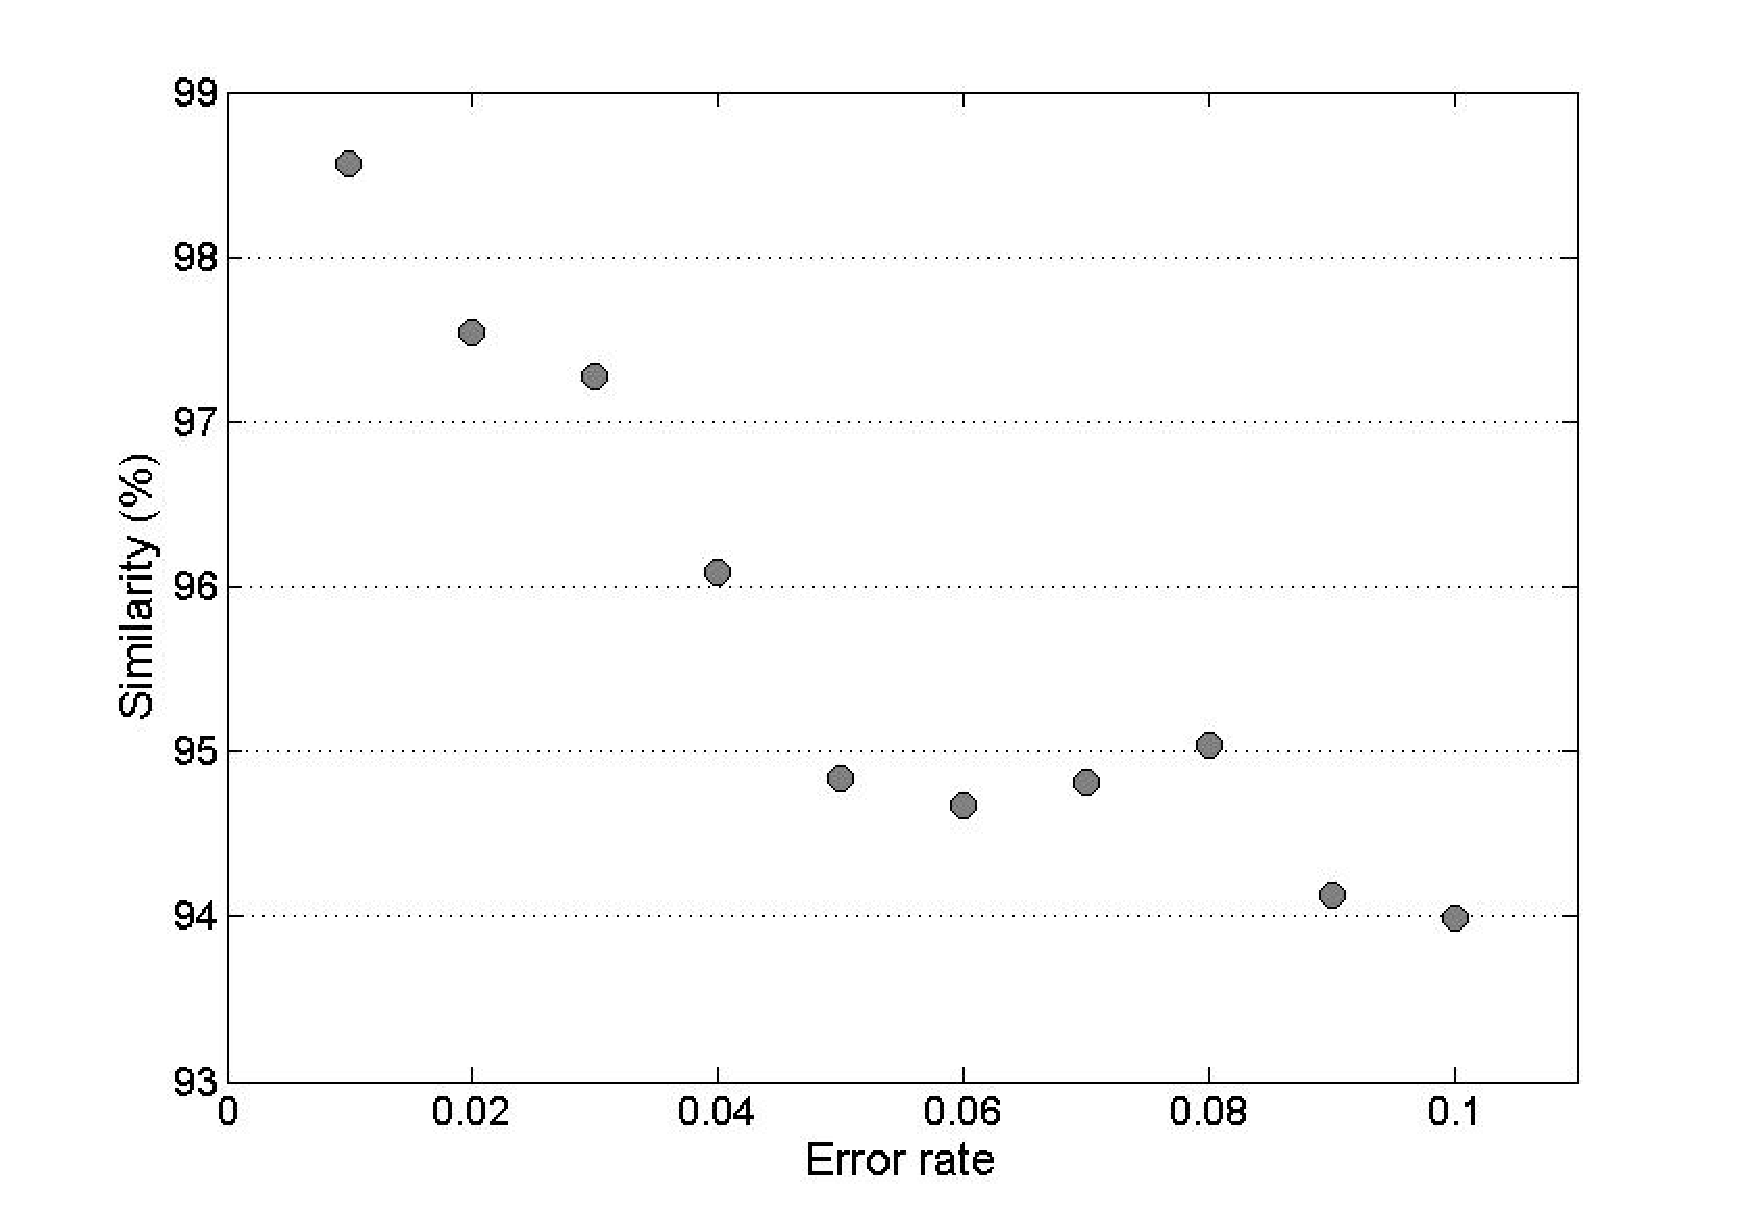
\includegraphics[width=0.6\textwidth]{./figs/error_correction.pdf}
  \caption{Error Tolerance for the Comparison Engine \cite{hu2012cmos}}
  \label{fig:err}
\end{figure}

%Implementation
\chapter{Testing}
\renewcommand{\baselinestretch}{\mystretch}
\label{chap:Testing}
\section{Overview}
%\setlength{\parindent}{0pt}
The testing of this system split into a logical correctness test; using multiple tools to identify any errors in the execution of the system, and a robust resource utilisation test. A number of tests with different parameters will be introduced in the testing section with their results shown in tables and figures below. Each of these tests will then be discussed in the evaluation section comparing the solution to the benchmark code that runs in simulation provided at the start of the report as well as other solutions that were discussed in the related work section. 

\section{Logical Verification}
The original comparison engine was made available as the basis for this project written in hardware description language VHDL, it works fully running under simulation in Modelsim. For the purposes of this project that code is used as a golden standard and later as a benchmark. Any bit error inconsistencies in the results are treated as errors. The design of this project was specifically organised such that there should be bit-wise consistency between the provided code and the implemented solution. It is important to note however, there are some limitations on this with regards to the non-deterministic effects introduced by clock skew across multiple devices and data transfer errors. Test data is inserted to both the simulation and the hardware implementation, both results are written out to text files in the same format. This text file is then checked for binary equality. 


A MATLAB version of the algorithm was also made available, however this produces different bitwise results, measuring the integer distance in overlaps rather than the bit-distance. As a result this was not suitable for verification. 


The full testing procedure consisted of varying several parameters, fitting from 5 to 12 pixels per device, testing read lengths of up to 1000 base pairs and changing the local library parameters to control the level of sensitivity the comparison engine. Having fully tested the FPGA based implementation it was found to produce correct results under the following set of test conditions. 

\begin{table}[!h]
\centering % used for centering table
\begin{tabular}{c c c c c c} % centered columns (4 columns)
\hline\hline %inserts double horizontal lines
Read Length & Genome Length & Pixel Count & FPGA Count & Library Size & Correct\\ [0.5ex] % inserts table 
%heading
\hline % inserts single horizontal line
50 & 113 & 5 & 1 & 5 & Yes \\ % inserting body of the table
400 & 1500 & 9 & 1 & 5 & Yes \\% [1ex] adds vertical space
400 & 3000 & 27 & 3 & 5 & Yes \\% [1ex] adds vertical space
400 & 3000 & 27 & 3 & 3 & Yes \\% [1ex] adds vertical space
400 & 3000 & 27 & 3 & 10 & Yes \\% [1ex] adds vertical space
1000 & 2000 & 20 & 2 & 10 & Yes \\% [1ex] adds vertical space
1000 & 10000 & 36 & 3 & 10 & Yes \\% [1ex] adds vertical space
\hline
\end{tabular}
\caption{Validation Results} % title of Table
\label{table:nonlin}
\end{table}


All parameters not listed were set as default as listed in appendix \ref{App:default}. 



\section{Performance Characteristics}
\subsection{Resource Usage}
The performance characteristics of the comparison engine can be measured in different metrics, all of which have significant practical meanings; logic utilisation, memory utilisation, clock frequency, and cycle count. A derived measurement of cumulative speed will also be shown, derived from the clock speed and cycle count measurements.

\subsubsection{Logic Utilisation}

Logic utilisation measures how much of the FPGA device is used by a given circuit and in the case of the comparison engine, is the limiting factor for how many pixels can fit on a single device. This measurement will be compared to the simulated implementation (referred to as the benchmark) in order to show how all of the data communication and control logic has increased the design. The ideal for this metric is to keep the logic utilisation as low as possible. In order to draw this comparison a number of parameters will be changed and the logic utilisation recorded. Ordinarily, due to the size of the FPGA this comparison would be very limited as the provided code would only work on a single device, in order to draw a good comparison of logic utilisation at the same computational level, a larger FPGA based on the same technology will be used for comparison. A discussion of the true achievable computational power will follow later. The full set of results are listed in \ref{table:logic}. For these tests identical compilation settings were used to guarantee the comparison were valid, and Altera CYCLONE III devices were used.

As a separate analysis of the resource utilisation, figure \ref{table:single} shows a break down of the resource utilisation of each sub-block. This shows the IO controller, built as part of this project's implementation uses around 2,700 logic elements, this translates to around 1-2 pixels worth of logic. This is cost of being able to scale across multiple FPGAs. Effectively the area available for pixels on the DE0 device is reduced by 2,700 logic elements but multiple FPGA's space becomes available. To further quantify this, the logic usage of various numbers of pixels was plotted. This is shown in figure \ref{fig:fpgacount}, it shows that the control logic introduces around a 1,000 logic element overhead for small pixel counts. At the larger pixel count, routing had a significant effect and the interconnection of the control logic caused bad scaling in the routing.



\begin{table}[!h]
\centering % used for centering table
\begin{tabular}{c c} % centered columns (4 columns)
\hline %inserts double horizontal lines
\hline
Sub-Block & Logic Elements\\  % inserts table 
\hline
Global Controller & 158 \\
Pixel Array & 12,047 \\
IO Controller & 2,272 \\
Scheduler & 192 \\
UART & 85\\
%heading
\hline
\end{tabular}
\caption{Resource Utilisation of a single Master processor with 9 pixels} % title of Table
\label{table:single}
\end{table}


\subsubsection{Memory Utilisation}
Similarly to logic utilisation, memory utilisation measures how much of the device resources are used by the design. As covered in the analysis of Y Hu's comparison engine, memory utilisation was very low for this algorithm. For this reason less importance was placed on minimising its usage. To quantify this, when over 80\% of a device's logic was used, less than 1\% of the onboard memory was used. The memory utilisation is affected by a sub-set of the parameters, read length, pixel count, and library size. These parameters set the size of the local FIFO buffers. The main priority with memory utilisation is only to ensure that the memory doesn't not scale significantly worse than the logic element utilisation. This will be discussed later in the evaluation section.


\vspace*{\fill}


\begin{sidewaystable}[p]
\centering % used for centering table
\begin{tabulary}{\textwidth}{C C C C| C C| C C C C}% centered columns (4 columns)
\hline\hline %inserts double horizontal lines
Read Length & Genome Length & Pixel Count & Library Size & Benchmark Logic Elements & Benchmark Memory Bits & Cluster Size & Implementation Logic Elements & Implementation Memory Bits \\
\hline 
% inserts single horizontal line
50 & 113 & 9 & 5 & 10,608 & 4,096 & 3 & (5,808)~(5,175) & (5,620)~(4,532)\\
50 & 113 & 15 & 5 & 17,564 & 4,096 & 3 & (7,946)~(8,230) & (6,612)~(4,732)\\
50 & 113 & 27 & 5 & 31,697 & 4,096 & 3 & (14,097)~(14,021) & (8,908)~(5,140)\\
50 & 113 & 45 & 5 & 54,342 & 4,096 & 3 & (21,701)~(26,448) & (12,124)~(5,740)\\
50 & 113 & 99 & 5 & 116,496 & 4,096 & 3 & (44,825)~(48,578) & (22,732)~(7,548)\\
\hline
50 & 100 & 27 & 5 & 31,697 & 4,096 & 3 & (14,097)~(14,021) & (8,908)~(5,140)\\
50 & 1,000 & 27 & 5 & 31,697 & 4,096 & 3 & (14,097)~(14,021) & (8,908)~(5,140)\\
50 & 10,000 & 27 & 5 & 31,697 & 4,096 & 3 & (14,097)~(14,021) & (8,908)~(5,140)\\
\hline
50 & 2,000 & 27 & 5 & 31,697 & 4,096 & 3 & (13,404)~(14,021) & (8,908)~(5,140)\\
100 & 2,000 & 27 & 5 & 31,936 & 4,096 & 3 & (13,290)~(14,065) & (9,952)~(6,048)\\
200 & 2,000 & 27 & 5 & 32,191 & 4,096 & 3 & (13,448)~(14,045) & (11,872)~(7,848)\\
400 & 2,000 & 27 & 5 & 32,276 & 4,096 & 3 & (13,400)~(14,082) & (15,616)~(11,456)\\
800 & 2,000 & 27 & 5 & 32,604 & 4,096 & 3 & (14,122)~(14,593) & (22,960)~(18,664)\\
1,600 & 2,000 & 27 & 5 & 32,716 & 4,096 & 3 & (14,253)~(14,584) & (37,360)~(33,064)\\
\hline
50 & 400 & 27 & 3 & 29,490 & 4,096 & 3 & (13,341)~(12,967) & (7,348)~(5,084)\\
50 & 400 & 27 & 5 & 30,747 & 4,096 & 3 & (13,404)~(13,828) & (8,908)~(5,140)\\
50 & 400 & 27 & 10 & 37,165 & 4,096 & 3 & (16,212)~(16,151) & (12,820)~(5,284)\\
50 & 400 & 27 & 20 & 47,831 & 4,096 & 3 & (20,891)~(20,116) & (20,668)~(5,580)\\
\hline 
50 & 400 & 40 & 5 & 50,513 & 4,096 & 1 & (58,609)~(N/A)~~~ & (13,896)~(N/A)\\
50 & 400 & 40 & 5 & 50,513 & 4,096 & 2 & (28,284)~(26,957) & (11,904)~(6,240)\\
50 & 400 & 40 & 5 & 50,513 & 4,096 & 4 & (15,084)~(14,116) & (10,888)~(5,240)\\
50 & 400 & 40 & 5 & 50,513 & 4,096 & 5 & (12,623)~(10,931) & (10,696)~(5,040)\\
50 & 400 & 40 & 5 & 50,513 & 4,096 & 8 & (8,799)~(7,735) & (10,420)~(4,740)\\
50 & 400 & 40 & 5 & 50,513 & 4,096 & 10 & (7,442)~(5,958) & (10,336)~(4,640)\\
\hline
\end{tabulary}
\caption{Comparison of Logic Utilisation, Implementation listed as (Master)(Each Slave)} % title of Table
\label{table:logic}
\end{sidewaystable}

\begin{figure}[p]
  \centering
  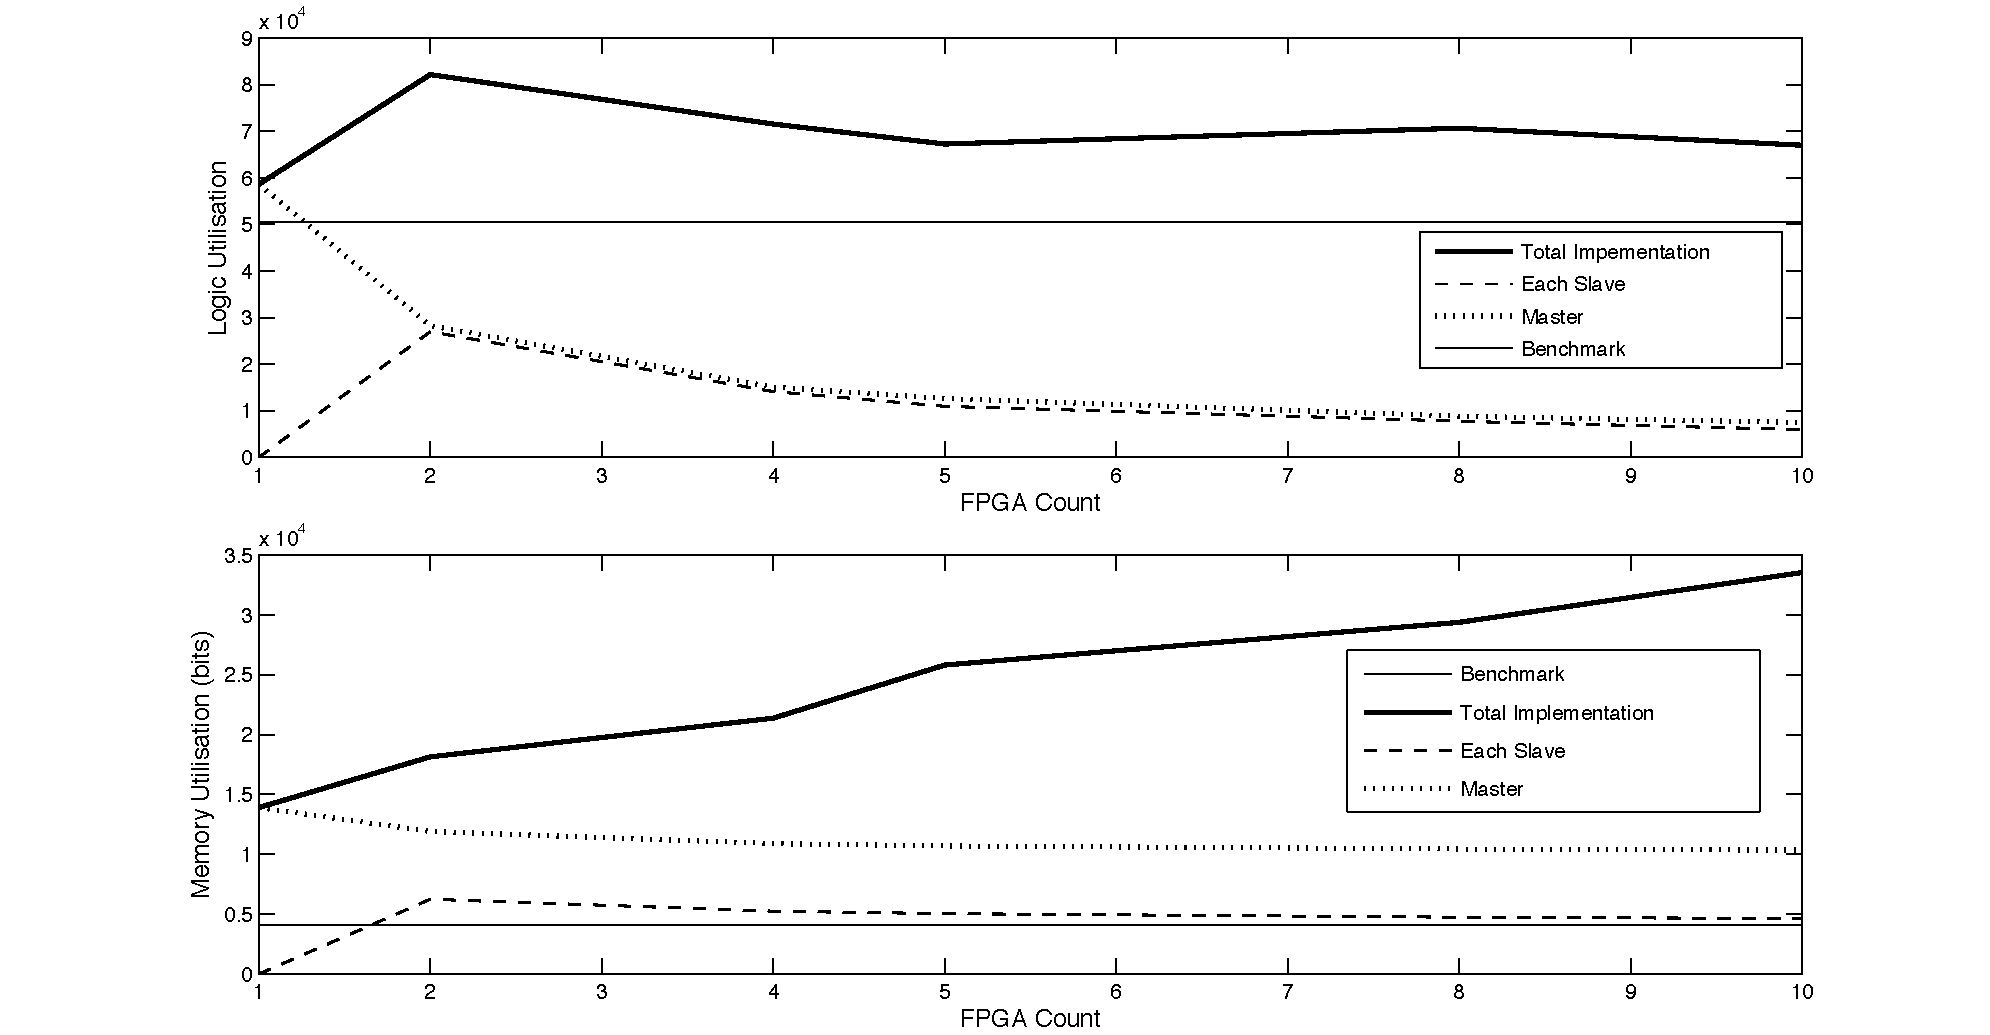
\includegraphics[height=0.4\textheight]{./figs/eps/fpga_count.pdf}
  \caption{Resource Utilisation Scaling with Device Count}
    \label{fig:fpgacount}
\end{figure}
\begin{figure}[p]
  \centering
  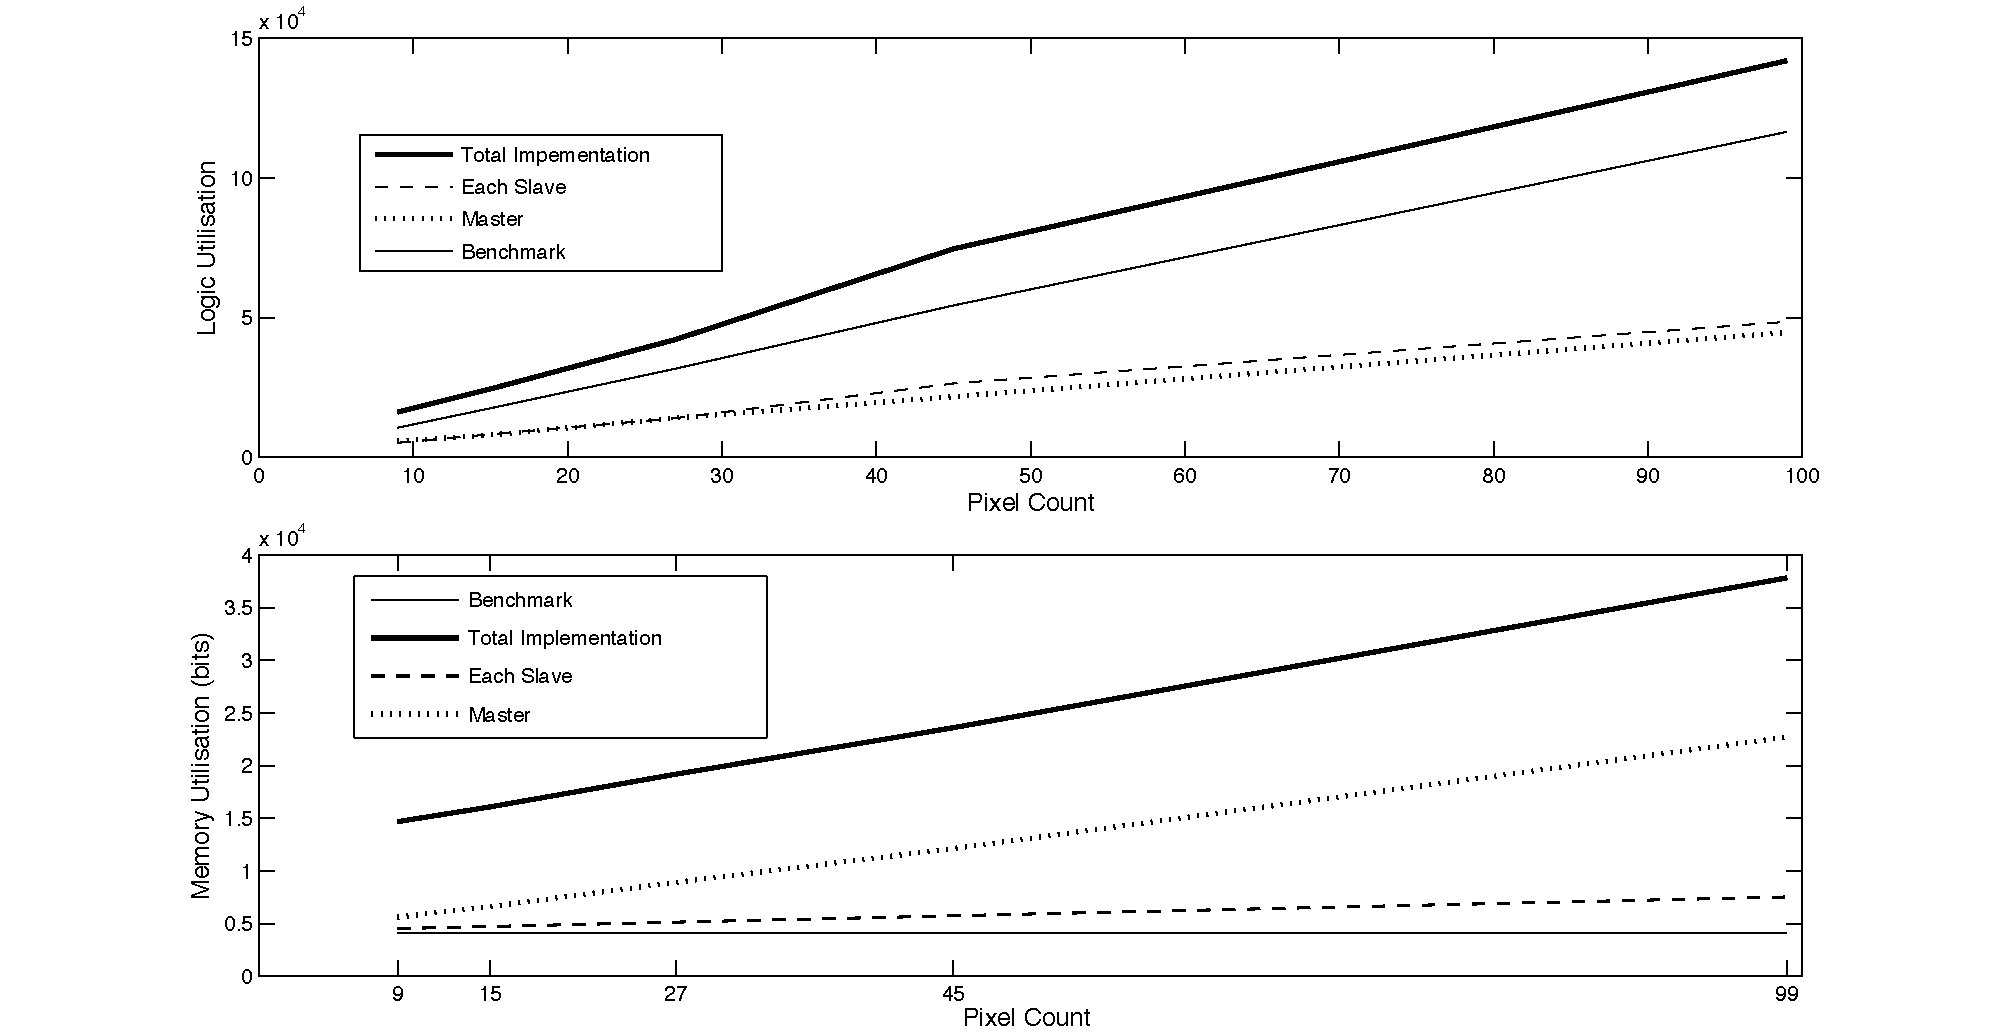
\includegraphics[height=0.4\textheight]{./figs/eps/pix.pdf}
  \caption{Resource Utilisation Scaling with Pixel Count}
    \label{fig:pix}
\end{figure}
\begin{figure}[p]
  \centering
  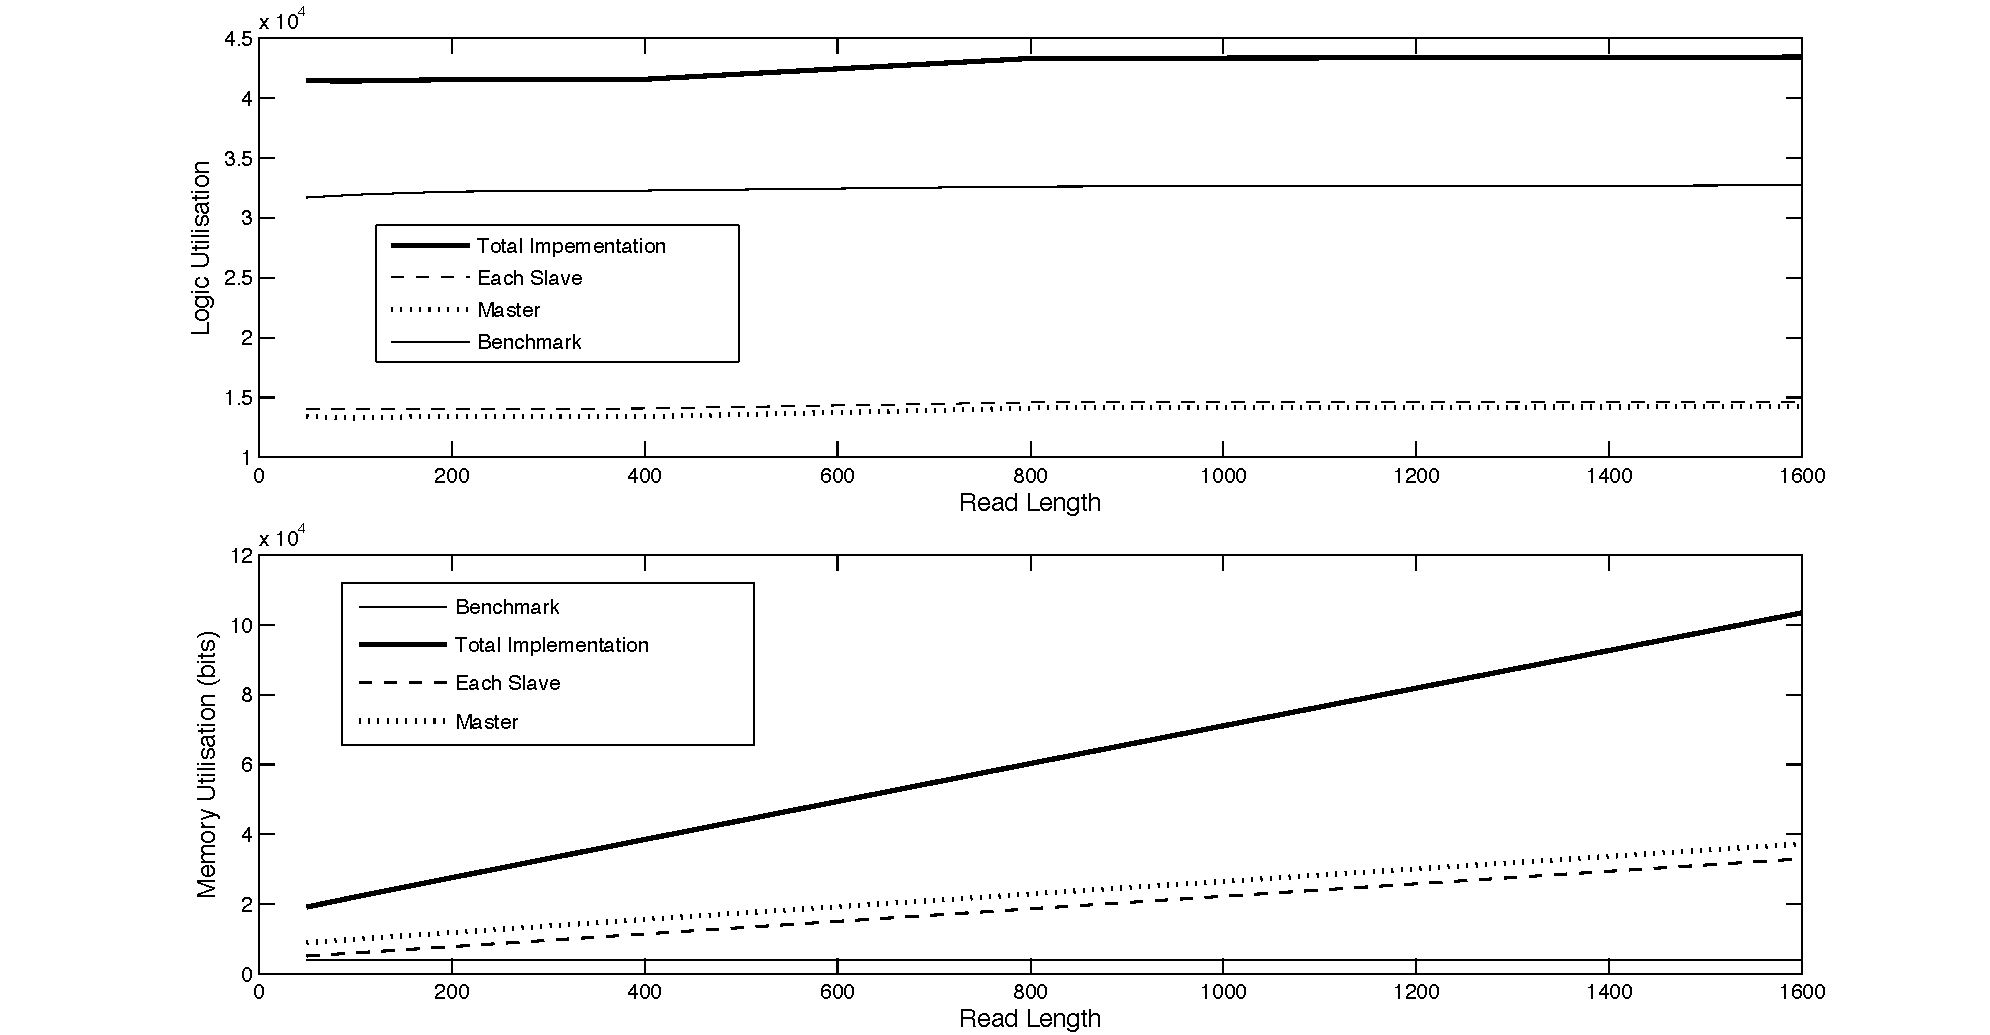
\includegraphics[height=0.4\textheight]{./figs/eps/read_length.pdf}
  \caption{Resource Utilisation Scaling with Read Length}
    \label{fig:read}
\end{figure}

\begin{figure}[p]
  \centering
  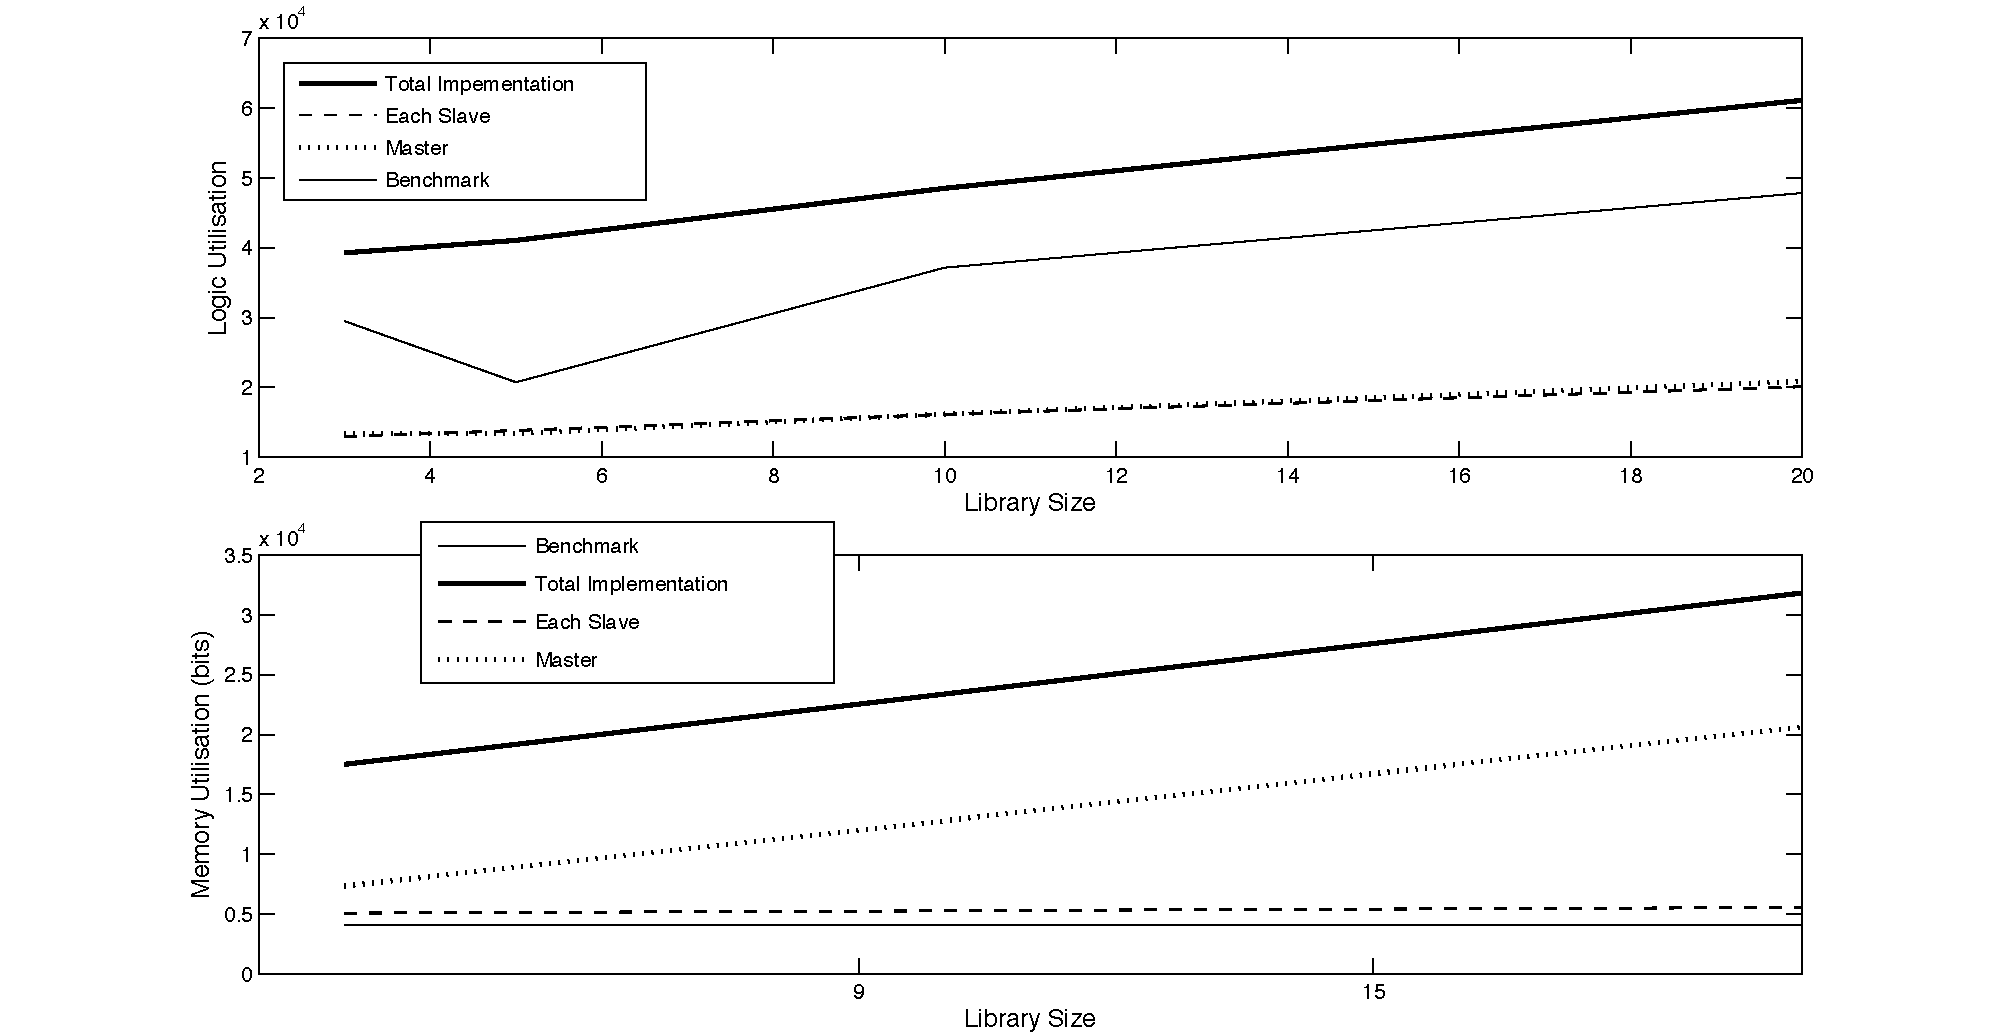
\includegraphics[height=0.4\textheight]{./figs/eps/lib_size.pdf}
  \caption{Resource Utilisation Scaling with Library Size}
    \label{fig:lib}
\end{figure}

\pagebreak
\subsection{Speed}
\subsubsection{Clock Frequency}
Clock frequency is one part of the equation for determining how fast the comparison engine can produce results. In the background section the clock speed of a single pixel was measured within the context of the process. Individually a pixel can reach 40.6~MHz, however within any full design drops to 33.1~MHz. In the implementation section however, more limitations were discussed for clock speed, due to the relatively long wiring between FGPAs and the shared clock domain. Within the calculations there a theoretical 260MHz could be reached, which far surpasses the local limitations. In this section the clock speed will be increased from 1~MHz to a full 33~MHz in practical tests and any bit errors in the results will be noted.



\subsection{Cycle Count}
Cycle count is a term which refers to how many clock cycles are required for a full comparison cycle between pieces of a string to happen. In the case of this algorithm there is a new comparison cycle after each new piece of pixel data arrives. This algorithm consists of two stages, the first where data is clocked in and buffers are filled, and the second where the buffers are filled and pixels are forwarding data. This second stage is the vast majority of the  processing time of the algorithm and therefore is the most important part to measure. In order to count the number of cycles, simulation data will be used, as measuring a single comparison cycle on the device is practically impossible. The way the algorithm executes is such that the cycle counts in simulation and on device should be identical. This data is shown in figure \ref{fig:wave}. This simulation was conducted as a comparison between 9 pixels in the benchmark code, and 9 pixels split across 3 devices on the 25th comparison cycle of a 50 read length sub-sequence.

\begin{sidewaysfigure}[!h]
  \centering
  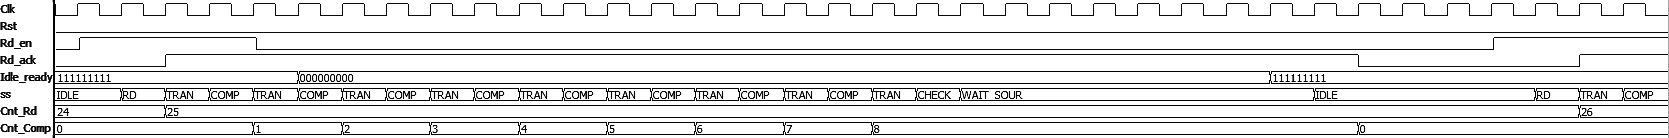
\includegraphics[width=\textheight]{./figs/provided.png} 
  \vspace*{4em}
 
   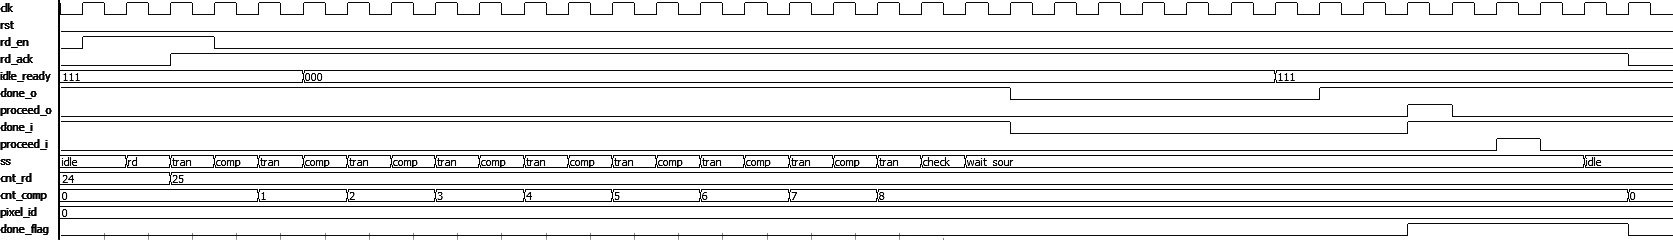
\includegraphics[width=\textheight]{./figs/MFPGA.png}
  \caption{Single Comparison Cycle. Left: Single FPGA Simulation; 29 Clock Cycles per Comparison Cycle. Right: 3 FPGA Cluster Simulation; 35 Clock Cycles per Comparison Cycle}
  \label{fig:wave}
\end{sidewaysfigure}

\subsection{Cumulative Speed}
As well as measuring the achieved frequency and the cycle count, it is important to look at the total speed of the algorithm. This can be done in two ways, the first is measuring the core speed of the algorithm, using the data provided by the clock frequency and cycle count. The second is to measure the total time between sending data to the hardware accelerator and receiving the full result library. The first can be done analytically with the data collected in the previous subsections; the time per comparison versus the clock speed.

\begin{align*}
\text{Comparison Rate} &= \frac{\text{Comparisons in Parallel} \times \text{Clock Frequency}}{\text{Cycles per Comparison}} \\
&= \frac{27\times 31\times 10^6}{35} \\
&= 23~\text{Million Comparisons per Second}
\end{align*}

One comparison occurs for each element of the string, and so for a 50 read length sample, 478 000 comparisons per second can be achieved. It is important to note though, this is only theoretical throughput. Data communication with the FPGA is a significant portion of the time, and this is best measured through practical testing. 


These practical tests can be carried out by using timers in the python host software to measure and report the time taken to do the full comparison and read out results. This takes into account all possible causes of delay and gives a much more accurate picture of the processing speed of the algorithm on this specific cluster.

This testing was done by sending overlap data to the device and receiving the result data 5 times within a timing section. The time measured was then divided by 5 to get the speed of a single set of comparisons. Various read lengths were run in order to see the effect of scaling the pixels to longer problems. 

The results of this test are listed in figure \ref{table:speed} with a pixel count of 27, and FPGA count of 3.  In order to minimise the impact of noise each measurement is an average of 10 runs of the algorithm, due to the nature of the program there should be no initial run cost. Only the comparison is being measured for speed, any data translations on the host side are not accounted for as in a full tool-chain these would vary significantly.


\begin{table}[!h]
\centering % used for centering table
\begin{tabular}{c c c c c c} % centered columns (4 columns)
\hline\hline %inserts double horizontal lines
Read Length & Genome Length & Library Size & Time (ms)\\ [0.5ex] % inserts table 
%heading
\hline % inserts single horizontal line
25 & 600 & 5 & 25\\ % inserting body of the table
50 & 600 & 5 & 31\\ % inserting body of the table
75 & 600 & 5 & 43\\ % inserting body of the table
100 & 600 & 5 & 59\\ % inserting body of the table
200 & 600 & 5 & 123\\ % inserting body of the table
400 & 600 & 5 & 229\\ % inserting body of the table
\hline
\end{tabular}
\caption{Practical Speed Tests} % title of Table
\label{table:speed}
\end{table}



 %Evaluation
\chapter{Evaluation}
\renewcommand{\baselinestretch}{\mystretch}
\label{chap:evaluation}
\section{Overview}
This evaluation section will look at the results of the tests designed in the previous section, producing metrics of exactly how fast and scalable this implementation is. Comparisons will be drawn against the benchmark system noting any differences in resource profile and speed. In the later section the algorithm will be considered in terms of real genomes and the size of this problem set as well as comparing the processor with other algorithms that were introduced in the related work section.
%\setlength{\parindent}{0pt}
\section{Comparison to Benchmark Algorithm}
\subsection{Resource Usage}
The memory utilisation tested in the performance characteristics section showed that memory usage scaled up proportional to the read length for the algorithm. This is expected due to the design of full read length sized FIFO memory storage. It can be noted however, that even read lengths of 1,600 gave only 37,360 memory bits, less than 20\% of the memory available on the DE0 FPGA. This scale of read length is significantly above the maximum lengths achieved with current pyrosequencing techniques, the maximum of which are only 1,000. As a result it's perfectly safe to allow full sequence buffering, which removes any risks from having a slower throughput in the comparison engine that the input source. 

In terms of logic utilisation, figures \ref{fig:fpgacount}, \ref{fig:pix}, \ref{fig:read}, \ref{fig:lib} show that the implementation uses around 4 thousand logic elements for the control and interface logic on each FPGA. This equates to around 2 pixels on an average device. As a result, the increase in processing power when moving from one device to two effectively $2\times \text{pixel count} - 4 $, and this overhead does not increase on a per device basis when adding more devices above this. This means that moving from a four device cluster to a five device cluster does not increase the logic on the original four devices at all, although memory usage increases marginally on the master. This makes the design particularly scalable in terms of resources.

When looking at how logic usage scales with pixel count, it can be seen from figure \ref{fig:pix} that the relationship is linear. Each pixel adds around 1,500 logic elements to the design and this relationship does not change depending on how many devices are used. This is the type of scaling that was expected and is ideal for maximising parallelism. It is important to note however that increased pixels does not necessarily directly relate to increased processing power as algorithm speed may be impacted.


Whilst it's theoretically possible to scale up the number of devices quite significantly, moving to dozens of devices before the clock skew issues would lower the clock frequency, this is still not the scale of the massively parallel operation the detection devices work on. Instead, larger devices such as the Terasic CYCLONE V GX development kit, would be able to massively scale up the computational power. As well as dedicated clock ports, the High Speed Mezzanine Connectors (HSMC) give the opportunity to increase the inter-FPGA communications which was cited as a key limitation in the hardware design section. Each of these devices is capable of fitting in the order of 100 pixels based on the tests shown earlier. As such, a large cluster of these devices would be capable of comparing thousands of pixels of data in parallel. It is important to note however, this is still not of the order of the very highest density chips. 

The scalability of the algorithm in terms of how many sequences can be shared between pixels and therefore how many parallel calculations can be done is a severe limitation. The number of inter-FPGA communication pins are always a hard limit, and with 30 pins required for the data IO communication, the number of pins required for the ring network can often be a limiting factor. This is therefore likely to be a key motivating factor when choosing hardware on which this algorithm can be implemented. There are solutions to this problem however, like the HSMC ports mentioned earlier. This does not prevent more pixels to be used on a single device however, and for this reason, the approach of smaller pixels with more comparison cycles may be necessary. The inter-pixel communication can be lowered by reducing the comparisons in parallel, this pays off both in number of inter-device connections as well as simplifying the logic of each pixel and therefore fitting more pixels per device. This does negatively impact the number of comparison cycles that need to be done however, and a balance must be made. This would normally be done by identifying the number of pixels absolutely necessary and the absolute maximum inter-device ports available. 


\subsection{Speed}


On smaller FPGAs such as the DE0 that was used for testing, only around 9 pixels can be fitted on a single device. This meant the 3 device cluster was capable of running a 27 pixel array, with speed of comparison as short as 31ms for the full comparison. This is equivalent to 478,000 comparisons per second making this array very powerful. The advantage of this system is the massive parallelism, an all against all comparison has a computational complexity of $O(n^2)$. For large n this becomes very slow, however for large n, a larger device can be used and the computation time scales with $O(\frac{n^2}{m})$ where m is the number of pixels. This significantly speeds up the operation. 


Another important element of speed is the effectiveness of adding an FPGA delay, as discussed earlier, a each extra FPGA device slows the cycle count by 2 cycles. Ignoring the effect of clock frequency, as long as the number of pixels per FPGA is greater than 2, an extra device will always increase processing power. However, clock frequency cannot be ignored, as all devices must work from the same clock, and whilst the path from one FGPA to another may not increase, attempting to keep the path of the clock the same to all devices would be extremely difficult. This means there would be clock skew between devices which limits how fast the clock frequency may be. As a result of this the best method for this algorithm is small clusters of high-powered devices. 


As discussed in the motivation section, the detection chip is using chemical processes to sequence the DNA which is significantly slower than the processing speed of a CMOS chip. The detection time period of around 4~s is orders of magnitude slower than the comparison engine, with can operate with a clock period of as little as 32~ns. The time to do a single comparison cycle has been shown to take $N + 2T $ where N is the overlap count and T is the number of FPGAs in the array. These measurements show that the comparison engine is more than capable of operating at speeds much faster than the detection chips. This is not enough however, for real-time processing. An important element of the comparison engine is the number of parallel comparison engine pixels that can be used within the circuit. The scale of the comparison engines pixels is no where near enough to allow true real-time stream processing of the detection chip data. In order to achieve this directly, modifications would have to be made to the algorithm as covered in the future work section.

\section{Comparison to Existing Technology}

In the testing section of the report figure \ref{table:speed} the speed of the algorithm was shown for varying read lengths with 27 pixels. At a read length of 50 the comparison engine processed ($27^2$) comparisons in 31~ms or $42~{\mu}s$ per comparison. It is possible to compare this to the assembly speeds of the algorithms discussed in the related work section. 

In the paper comparing sequence assemblers it was found the quality of recombined sequences generally did not improve about 40x coverage depth, meaning that the short reads defined the full sequence 40 times \cite{lin2011comparative}. For genome lengths of 4.6~million in the case of E.Coli, this would mean $\frac{4.6\times 10^6 \times 40}{50} = 3.68~\text{million}$ reads with read length 50. When taking into account these facts, the total estimated time for the DE0 FPGA cluster to do this comparison would be $(3.68\times 10^{6})^2 \times 42 \times 10^{-6} = 5.6\times10^{9}~\text{s}$. This can be compared to the times listed in figure \ref{fig:comp}, for the other comparison engines. unfortunately this indicates that fast sequencing for full genomes is unrealistic on a 3 DE0 based cluster. This however, is unsurprising as this cluster is extremely low cost when compared to the hardware set up for testing. The testing of the other solutions was conducted on a cluster of 8 computers each of which had 2 quad-core 2.4~GHz processors. This meant that each of these solutions was using 64 processors in parallel to achieve these results. As a result it is unrealistic for this hardware to compare to those benchmarks. When considering a true comparison with this massive assembly problem a more powerful cluster would need to be built.



A cluster of only 3 DE0 boards would more realistically work in real-time for much smaller data sets, in the order to 10kbp, where complete comparison for a 40 times coverage 50 read length would only take 1.68~s. The cluster built in this project was an extremely small implementation of the cluster design, and is unsurprisingly less powerful than the system that was used to test the other algorithms. In order to look at the how a larger cluster would manage larger problem sets, the scalability of the hardware must be analysed.


\subsection{Scalability of hardware}

Predominantly, the limits on the cluster are related to the number of devices used. As discussed earlier, each additional device in the cluster adds a 2 cycle delay per comparison, when scaled across large numbers of devices this forms a limiting constraint on the speed of comparisons. Assuming perfect scaling of the algorithm in terms of frequency, data availability of clock speed the algorithm still tends to a speed limit, this is shown in figure \ref{fig:scale}.

\begin{figure}[!h]
  \centering
  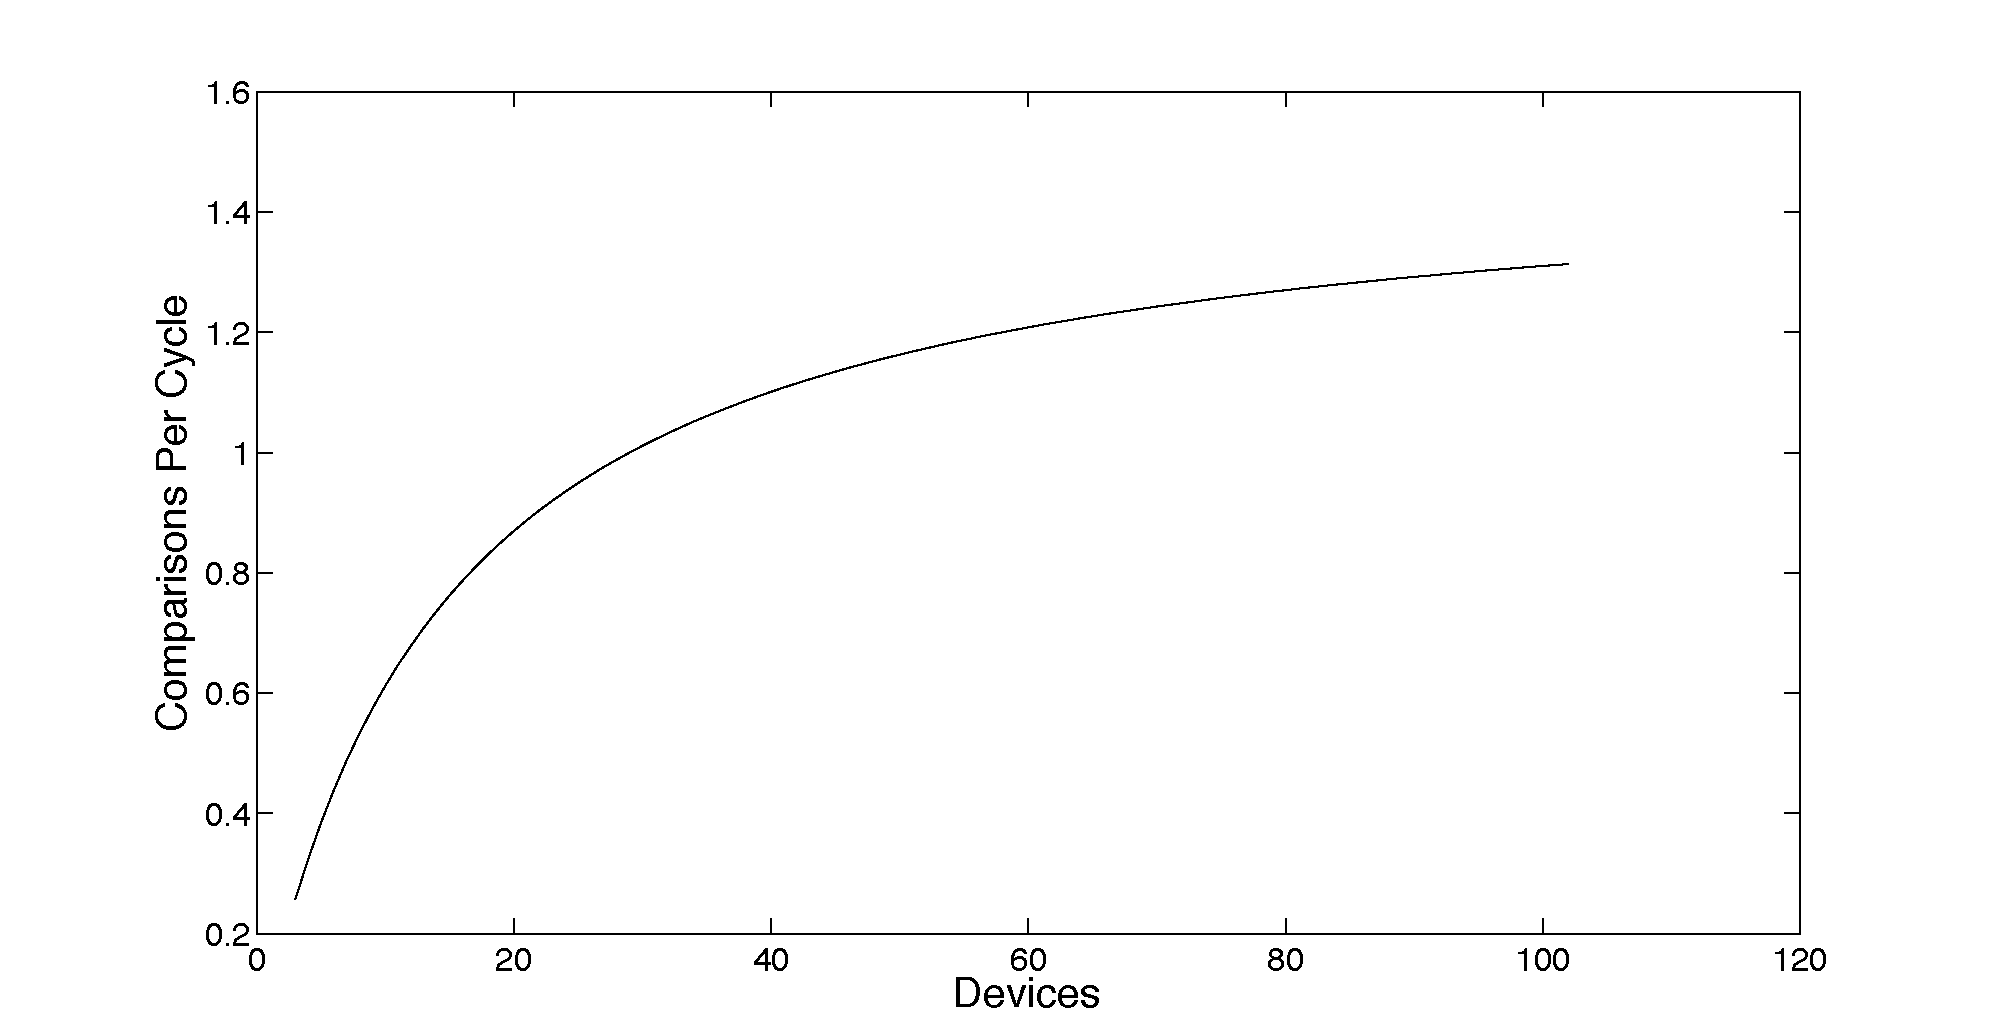
\includegraphics[width=0.7\textwidth]{./figs/scalability.pdf}
  \caption{Scaling of Algorithm with Cluster Size}
    \label{fig:scale}
\end{figure}

This is a hard limit on the scalability of the algorithm due to the delay introduced by the inter-device communication. This only occurs for a very large size of cluster and other factors are likely to come into effect before this. This pattern is  an important factor in scaling the algorithm, as earlier the linear scaling of pixels was discussed in terms of logic utilisation. As logic usage increases, the pixels must be spread across multiple devices, as can be seen in figure \ref{fig:scale} this tends to a limit as the cluster size increases. This means that whilst increasing pixel count per device linearly increases processing power, increasing number of devices tends to a limiting factor due to the length of the comparison cycle increasing. 


The main factor limiting the scalability of this hardware is the clock skew across devices. A shared clock design is naturally limited to how many devices can share the clock synchronously. This largely depends on device hardware, as a clock source coming in to a board via a normal GPIO port is not a high quality clock source, as such it is likely to be skewed and difficult to synchronise across devices. In contrast, higher quality devices have custom clock inputs using Subminiature A connectors designed specifically for the purpose of high quality external clocks. 


An important factor in the scalability of this solution is how efficiently the design can be used to tackle larger problem sizes. This introduces a problem with the comparison engine, it is of comparable speed to the other algorithms presented, especially when considering the disparity in hardware resources. However, scaling the number of comparisons done on the current device is not as simple as doing multiple comparison cycles at full speed. The comparison engine is designed to do a comparison shown in the matrix below, where n is the number of pixels on the cluster.
\begin{center}
$\text{Comparison Matrix} =  \begin{pmatrix}
  F(a_{1},a_{1}) & F(a_{1},a_{2}) & F(a_{1},a_{3}) & \cdots & F(a_{1},a_{n}) \\
  F(a_{2},a_{1}) & F(a_{2},a_{2}) & F(a_{2},a_{3}) & \cdots & F(a_{2},a_{n}) \\
  F(a_{3},a_{1}) & F(a_{3},a_{2}) & F(a_{3},a_{3}) & \cdots & F(a_{3},a_{n}) \\
  \vdots  & \vdots  & \vdots & \ddots & \vdots   \\
  F(a_{n},a_{1}) & F(a_{n},a_{2}) & F(a_{n},a_{3}) & \cdots & F(a_{n},a_{n})
 \end{pmatrix}
$
\end{center}

It is important to notice however, that with the current algorithm it is impossible to only do some of these comparisons, they must all be done in lock-step. As a result performing a comparison of a larger number of sequences is difficult, as a  larger square comparison matrix cannot be formed of repeated smaller square matrices without significant repetition of the same work. This makes using the parallel comparison engine poorly suited to processing larger problemes. In the next section we discuss a method that could be adopted to solve this problem.  %Discussion
\chapter{Future Work}
\renewcommand{\baselinestretch}{\mystretch}
\label{chap:futurework}
%\setlength{\parindent}{0pt}

A primary goal of any future work would be a further scaling of this algorithm. The small scale cluster presented in this report showed the algorithm could successfully accelerate comparison computation. However, this technology could be significantly scaled to larger devices as well as a larger number of devices to further accelerate computation in a practical situation. For example, larger FPGA devices currently on the market would each be able to support on the order of a hundred pixels \cite{altcyc}.


Another avenue for future work was raised in the evaluation section. Having introduced the concept of the comparison engine as a matrix of overlap operations it is possible to decompose this system into a set of sub-systems. The ring network currently circulates the data in the pixels around once, comparing all data to each other. However, this could be extended simply to break the ring, feeding new data into the comparison system via the a break in the ring network. In terms of the comparison matrix this would allow computation of a rectangular matrix, a group of these matrices would then be able to combine to produce a single large square comparison matrix as shown below. 


\begin{align*}
\text{Comparison Matrix} &=  \begin{pmatrix}
  F(a_{1},a_{1}) & F(a_{1},a_{2})  & \cdots & F(a_{1},a_{2n}) \\
  F(a_{2},a_{1}) & F(a_{2},a_{2})  & \cdots & F(a_{2},a_{2n}) \\
  \vdots  & \vdots   & \ddots & \vdots   \\
  F(a_{2n},a_{1}) & F(a_{2n},a_{2}) & \cdots & F(a_{2n},a_{2n}) \\
 \end{pmatrix}  \\
 \text{Sub Matrix}_0 &=
 \begin{pmatrix}
  F(a_{1},a_{1}) & F(a_{1},a_{2})  & \cdots & F(a_{1},a_{n}) \\
  F(a_{2},a_{1}) & F(a_{2},a_{2})  & \cdots & F(a_{2},a_{n}) \\
  \vdots  & \vdots & \ddots & \vdots   \\
  F(a_{2n},a_{1}) & F(a_{2n},a_{2})  & \cdots & F(a_{2n},a_{n})
 \end{pmatrix} \\
\text{Sub Matrix}_1 &=  \begin{pmatrix}
  F(a_{1},a_{n+1}) & F(a_{1},a_{n+2})  & \cdots & F(a_{1},a_{2n}) \\
  F(a_{2},a_{n+1}) & F(a_{2},a_{n+2})  & \cdots & F(a_{2},a_{2n}) \\
  \vdots  & \vdots & \ddots & \vdots   \\
  F(a_{2n},a_{n+1}) & F(a_{2n},a_{n+2})  & \cdots & F(a_{2n},a_{2n})
 \end{pmatrix} \\
 \text{Comparison Matrix} &= \text{Sub Matrix}_0 \parallel \text{Sub Matrix}_1
\end{align*}

\normalsize
Using a broken ring network it is possible to feed more data into the comparison engine than there is number of pixels. Each usage of the comparison engine would then produce a rectangular matrix, with the width still set at the number of number of pixels, but the height set at an arbitrary size. 

In order to produce the full matrix of comparison data it is necessary then to either run the comparison engine multiple times, or run multiples comparison engines in parallel using the other pixel data as the home data for each pixel. Either of these solutions mitigates the problem of having a relatively small number of pixels per device by subdividing the problem. The solution of running the same comparison engine twice reduces cost but increases time, and doesn't allow the second run of the algorithm to exploit any delay in the detection. The second solution of multiple comparison engines in parallel works particularly well, as although it is increased cost, it increases parallelism further without the issues of clock speed and data transfer speed limits. This would be a suitable way of further increasing computation power easily. 


This change is an important advancement, as the current algorithm places requirements on which comparisons must happen in parallel, which means to decompose a large square comparison matrix into smaller square comparison matrices that are compatible with the algorithm requires some data to processed multiple times. This inefficiency is a significant problem in terms of the speed of the algorithm.

This modification to the algorithm could be done relatively simply, as much of the work has been done. Removing the link between number of pixels present and number of comparison cycles has already been done when scaling the algorithm to multiple FPGAs. The only significant work to do this would be a modification to the input data protocol as it currently only feeds data into pixels with their own current sequence.
 %Future Work
\chapter{Conclusion}
\renewcommand{\baselinestretch}{\mystretch}
\label{chap:conclusion}
%\setlength{\parindent}{0pt}
In conclusion, a comparison engine architecture has been successfully implemented on a cluster of FPGAs, with a full testing regime verifying its operation. Fitting up to 27 parallel processing units on 3 low-cost DE0 board the cluster significant success has been seen in the area of real-time processing. With tests showing a full set of all-against-all comparisons being carried out in only 31~ms the objective of producing a machine capable of real-time processing has been significantly fulfilled for small sized problem sets in the order of thousands of base pairs. This substantially fulfils the main objective of this project, with the deliverable framework of code and hardware set-up successfully built and documented.


The design of this multi-FPGA comparison system has successfully showed scaling computation across multiple devices. The ability to exploit the detection time of DNA detection circuitry was enabled through the implementation of a streaming interface and the use of full sequence buffering has been enabled with minimal effect on device size through the use of onboard memory. The device interface is completely platform independent with the use of a universal asynchronous receiver/transmitter block handling all external communications. The interface software also support multiple platforms, having been implemented in Python.

Limitations of the algorithm have been discussed with the impact of both implementation problems such as clock skew, and digital design limitations with the impact of a two cycle delay per FPGA. A practical approach to finding these limits involved both initial estimates using velocity factors of transmission wires, as well as practical tests with modifications to the onboard clock generator. There is a balance between the maximum achievable clock speed and number of devices within the cluster that must be found, as lowering clock speeds impact the power of the system significantly. For tests with small clusters the internal algorithm frequency limits of 31MHz proved to be a limiting factor, and theory dictates up to dozens of FPGAs could be used in a cluster before significant impact of inter-FGPA communication on clock speed. Values calculated in the implementation section indicated the cluster could be significantly extended before clock speed is lowered.


The multi-FPGA cluster overcomes the traditional limits of size on single chips. The interface logic introduces a roughly 4,000 logic element overhead which does not scale with algorithm size, and is relatively small compared to larger devices capable of fitting up to 100,000 logic elements on a single chip. This design favours small clusters of large devices forming clusters over large clusters of small devices. 

When comparing the algorithm with current sequencing solutions a significant difference in scale was found. The testing of other algorithms tended to focus on very high end hardware and as a result saw much better performance. This indicated that for a true real-time solution a more expensive FPGA cluster may need to be designed. Although considering the hardware available, the comparison engine has showed fast results for smaller problem sizes. 


Finally, further work was identified with a recommendation that a small change in the current structure of the algorithm could allow the processing of much larger data sets in a more efficient manner. The current all-against-all processing element structure has been shown to be limiting for large problem sizes due to the amount of repeated work that may be necessary when processing large data sets. %Conclusion



%%%%%%%%%%%%%%%%%%%%%%
% The reference list.%
%%%%%%%%%%%%%%%%%%%%%%

\renewcommand{\baselinestretch}{1}

% Note: put the bib style and bib file you use here.
\bibliographystyle{IEEEtran}
\bibliography{IEEEabrv,MyCollection}

%%%%%%%%%%%%%%%%%%%%%%%%%%%%%
% The end of reference list.%
%%%%%%%%%%%%%%%%%%%%%%%%%%%%% 
\fancyhead[RE]{\emph{References}}

\appendix
\renewcommand{\baselinestretch}{1.5}
\chapter{User Guide}
\label{App:UserGuide}

The comparison engine project consists of 3 parts; hardware, device logic, and host software. Using this system involves a number of steps initially setting up each part, and then a simple command line program to run the comparison.

\section{Getting the Code}
All code and resources for this project are available on request from jcr09@ic.ac.uk.

\section{Setting up the Hardware}

The first step required in using the comparison engine is to set up the hardware. This involves connecting the FGPAs together, this is done as detailed in the hardware section of the report (Section 1, Chatpter \ref{chap:design}). This requires connecting each FPGA to the next with ribbon cable as shown in the figures on the next page. Shown on the next page is the setup for the DE0 cluster. A UART must be connected to 1 FPGA, the master device. This is most commmonly done with a UART-USB connector such as the FTDI USB-RS232 cable listed in the bibliography here as reference \cite{FTDI}. Only the TX and RX connectors are needed, the flow control signals can be left unconnected.

 
\begin{figure}[p]
  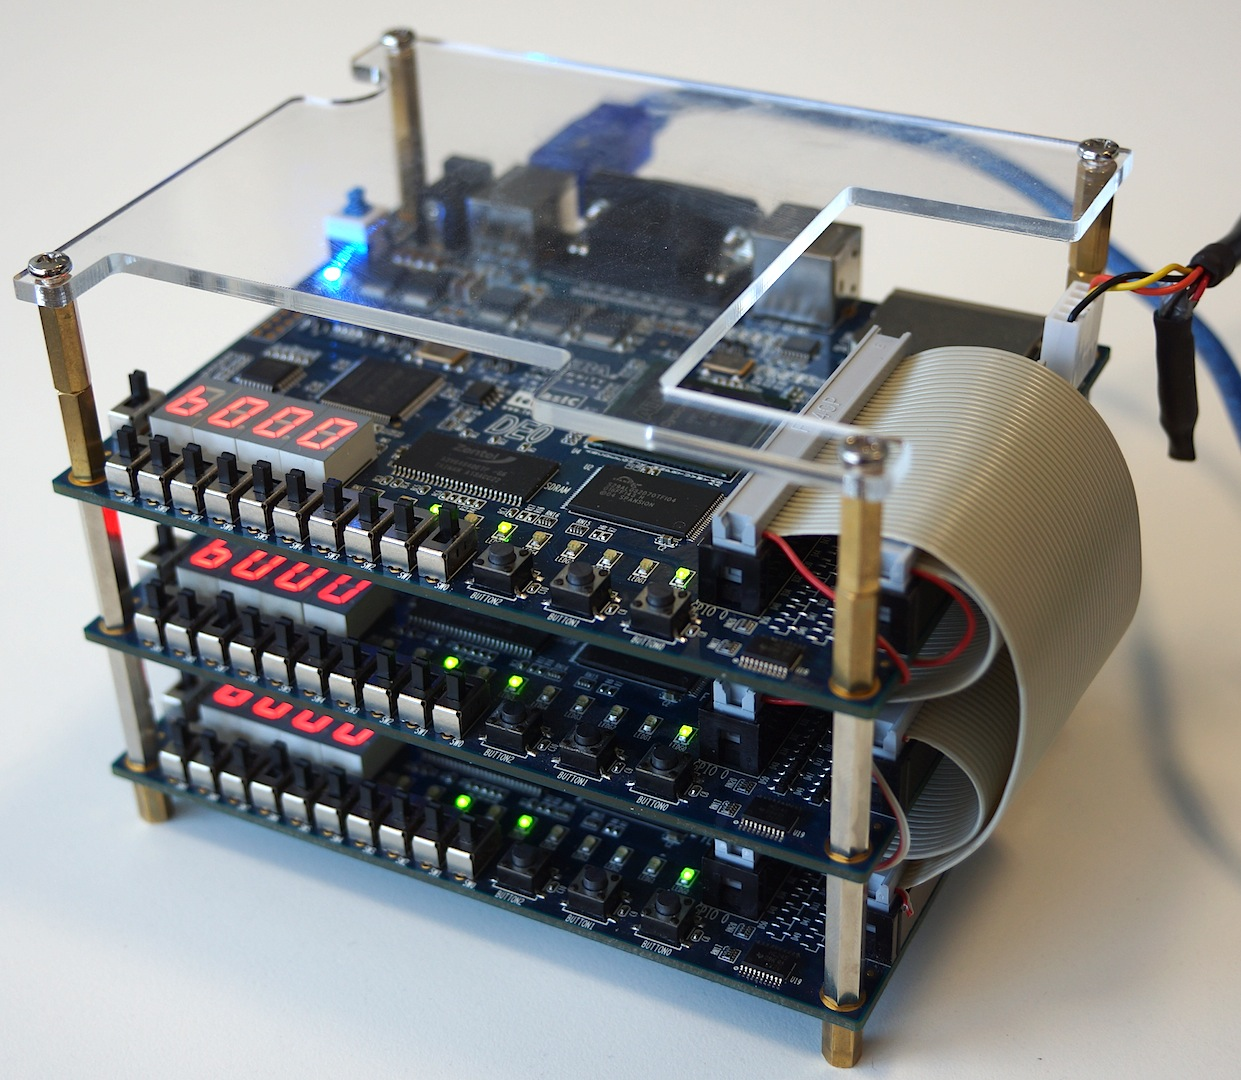
\includegraphics[width=\textwidth]{./figs/cluster.jpg}
  \caption{Hardware Implementation}
\end{figure}

\begin{figure}[p]
  \includegraphics[width=\textwidth]{./figs/interfpga.pdf}
  \caption{Inter-FPGA Communication Hardware Setup}
\end{figure}

\section{Programming the FPGA Devices}


The FPGA device images is the setup information that dictates how the FPGA functions. In order to do this, 2 images must be compiled. One image will go on the slave, one on the master. The master is the device that produces the clock and is connected to the UART as detailed earlier. This is done in the Altera Quartus II software with the two projects made available on request. 
\subsection{Customising the Algorithm}

Any customisations to read length, pixel count or genome length must be done with the devices images. These are all done in the Parameters.vhd file. In this file all settings can be customised, default settings are listed in appendix \ref{App:default}. Once these are modified the two images are compiled. 

If the hardware setup is non-standard the pin planner should be used to define which pins each port should be connected to. This is done on Assignments $>$ Pin Planner page using relevant data from the hardware datasheet generally available from the manufacturer. 


\subsection{Compiling the Images}

The majority of the compilation work is done by Quartus. The image is compiled by running the compilation, at which point an output SOF file is produced, this is an image that can be stored in the RAM of the FPGA device. This then needs to be converted to an image that can be stored permanently on the FPGA device (not cleared when power is lost). This is done using Quartus' converter by going to File $>$ Convert Programming Files... with settings stored in MASTER.cof and SLAVE.cof files. Once this is done, the Quartus programmer can be used to program the devices.


\subsection{Programming the Devices}

The devices are programmed in Programming mode entered by turning the power off, switching the programming switch shown in figure \ref{fig:de0} and turning power on with the USB BLASTER cable plugged in. Using the Quartus programmer (found in Tools $>$ Programmer) each device should be programmed with the POF image produced by the converter using the Active Serial mode. Once all devices have been programmed, each device should be returned to run mode using the switch and the reset should be pressed on the master device.

At this point the switches 6 to 9 should be set to the binary value indicating the order of the device in the cluster.

\textbf{\textit{NB. Once these tasks are complete the running of the comparison engine can be run as many times as wanted without reprogramming.}}

\section{Running The Comparison}

Having programmed the devices, it is now possible to run the comparison using the python script or program provided. This should be done from the command line, navigating to the location of the executable. The program should be run with the following arguments: Location of input file, number of pixels, read length. The input file should follow the format listed in Chapter 4 Section 3- Host Software. For example ``Testbench.exe dna.text 27 50''. This will trigger the comparison engine to run, returning the output data to a time stamped text file in the directory of the program. The output data will also be in the format listed in Chapter 4 Section 3. 
\renewcommand{\baselinestretch}{1.5}
\chapter{Host Interface Code}
\label{App:Host_Software}
\lstset{language=python, numbers=left, showspaces=false,
    showstringspaces=false, tabsize=4, breaklines=true, basicstyle=\tiny, captionpos=b, numbersep=5pt }
\begin{lstlisting}[frame=single,label=listing:IDT]
#!/usr/bin/python
import serial
import fileinput
import sys
import array
print(" \n------Comparison Engine Tester------")

if len(sys.argv) < 4:
	print("Please enter arguments: Filename, Pixel Count, Read Length")
	exit()
print("Requesting Comparison with :", sys.argv[2] , "Pixels, and Read Length of ", sys.argv[3], "\n")
PIXEL_COUNT = int(sys.argv[2])
READ_LENGTH = int(sys.argv[3])

source = open(sys.argv[1],"r")
print("Opened " , source.name)
data_in = []
for line in source:
	data_in.append(line)

a = 0
b = 0
c = 1
d = 0
TOTAL_DATA_COUNT = PIXEL_COUNT*READ_LENGTH
byte_size = int((TOTAL_DATA_COUNT+2)/4)
data_byte_array = bytearray(byte_size)

for i in range(0,TOTAL_DATA_COUNT-1,1):
	if(data_in[a][b] is "A"):
		data_byte_array[d] += 0*c
		#print("FOUND AN A!")
	elif(data_in[a][b] is "T"):
		data_byte_array[d] += 1*c
		#print("FOUND AN T!")	
	elif(data_in[a][b] is "C"):
		data_byte_array[d] += 2*c
		#print("FOUND AN C!")	
	elif(data_in[a][b] is "G"):
		data_byte_array[d] += 3*c
		#print("FOUND AN G!")
	else:
		print("------Found and invalid Character in input file, exiting...")
		exit()
	a += 1
	if a == PIXEL_COUNT : 
		a = 0
		b += 1
	c = c*2
	if c == 16:
		c = 1
		d += 1
#####UART INTERFACE
# print(data_in[4][0])
#
UART= serial.Serial()
UART.baudrate = 115200
UART.port = 'COM3'
UART.timeout = 5;
UART.open()
print("\nSerial Interface Settings: ",UART, "\n")

print("Written ",UART.write(data_byte_array), "Bytes to UART \n")
data_out = UART.read(493)
print("Received response from FPGA \n")

print(data_out)
source.close()
\end{lstlisting}

\renewcommand{\baselinestretch}{1.5}
\chapter{Comparison Engine Parameters}
\label{App:default}

\lstset{language=python, numbers=left, showspaces=false,
    showstringspaces=false, tabsize=4, breaklines=true, basicstyle=\tiny, captionpos=b, numbersep=5pt }
\begin{lstlisting}[frame=single]
-- file name: parameters.vhd
-- author: yuanqi hu
-- email: yuanqi.hu09@imperial.ac.uk
-- date: 23/08/2011
-- version: 1.0
-- abstract: this file list all the parameters need in upper level designs.
-- called by: all
-- revision history: Modified by James Rose for Multi-FPGA compatibility

LIBRARY ieee;
USE ieee.std_logic_1164.ALL;
USE ieee.numeric_std.ALL;

PACKAGE parameters IS

	--james added vars
	CONSTANT FPGA_COUNT        : INTEGER := 3;
	CONSTANT TOTAL_PIXEL_COUNT   : INTEGER := 27;
	-------------------pixel parameter----------------------
	CONSTANT GENOME_LENGTH         : INTEGER := 113;
	CONSTANT GENOME_WIDTH        : INTEGER := 7; -- width is the width needed to represent the number
	CONSTANT READ_LENGTH         : INTEGER := 50;
	CONSTANT READ_WIDTH        : INTEGER := 6;
	CONSTANT FIX_LENGTH          : INTEGER := 8;
	CONSTANT FIX_WIDTH         : INTEGER := 3;
	CONSTANT LOCAL_PIXEL_COUNT   : INTEGER := 9;
	CONSTANT LOCAL_PIXEL_WIDTH : INTEGER := 4;
	CONSTANT POOL_SIZE          : INTEGER := 5;
	CONSTANT redun             : INTEGER := 2;
	CONSTANT MAX_DISTANCE          : INTEGER := redun + 1;
	CONSTANT DISTANCE_WIDTH        : INTEGER := 3;
	CONSTANT OVERLAP_THRESH          : INTEGER := READ_LENGTH - FIX_LENGTH;

	-------------------ram parameter-----------------
	CONSTANT WORD_WIDTH : INTEGER := 2 * FIX_LENGTH;
	CONSTANT ADDRESS_WIDTH : INTEGER := 8;
	CONSTANT HOLD_TIME  : TIME    := 3 NS;
	CONSTANT SETUP_TIME : TIME    := 3 NS;
	CONSTANT WIDTH_TIME : TIME    := 20 NS;
	CONSTANT WP_TIME    : TIME    := 20 NS;

	-------------------timing parameter--------------
	CONSTANT PERIOD            : TIME    := 20 NS;
	-------------------buffer parameters------------
	CONSTANT BUFFER_SIZE       : INTEGER := GENOME_LENGTH * LOCAL_PIXEL_COUNT * 2 - 1;
	CONSTANT BUFFER_SIZE_BYTES : INTEGER := (GENOME_LENGTH * LOCAL_PIXEL_COUNT * 2 + 4) / 8;
	-- the following are some subtypes defined for the counters that need a few bits only
	SUBTYPE STABLE_INT_TYPE IS INTEGER RANGE 0 TO 1; --  WP_TIME/PERIOD+1;
	SUBTYPE NT_INT_TYPE IS INTEGER RANGE 0 TO 3; --  atcg four kinds of nucleotide
	SUBTYPE POOL_INT_TYPE IS INTEGER RANGE 0 TO POOL_SIZE;
	SUBTYPE RD_INT_TYPE IS INTEGER RANGE 0 TO READ_LENGTH;
	SUBTYPE PIXEL_INT_TYPE IS INTEGER RANGE 0 TO LOCAL_PIXEL_COUNT - 1;
	SUBTYPE FIX_INT_TYPE IS INTEGER RANGE 0 TO FIX_LENGTH - 1;
	SUBTYPE EDDI_INT_TYPE IS INTEGER RANGE 0 TO MAX_DISTANCE;
	SUBTYPE WAIT_INT_TYPE IS INTEGER RANGE 0 TO FIX_LENGTH + 1;
	SUBTYPE BASE_INT_TYPE IS INTEGER RANGE 0 TO redun + 1;
	SUBTYPE SHIFT_INT_TYPE IS INTEGER RANGE -redun TO redun;

	----------------------------------------------
	-- multiple dimension arrays 
	SUBTYPE OVERLAP IS UNSIGNED(LOCAL_PIXEL_WIDTH + READ_WIDTH - 1 DOWNTO 0);
	SUBTYPE BASE IS UNSIGNED(1 DOWNTO 0);
	TYPE ADDR_ARRAY IS ARRAY (NATURAL RANGE <>) OF UNSIGNED(ADDRESS_WIDTH - 1 DOWNTO 0);
	TYPE WORD_ARRAY IS ARRAY (NATURAL RANGE <>) OF UNSIGNED(WORD_WIDTH - 1 DOWNTO 0);
	TYPE OVERLAP_vect IS ARRAY (NATURAL RANGE <>) OF OVERLAP;
	TYPE DNA_SEQUENCE IS ARRAY (NATURAL RANGE <>) OF BASE;
	TYPE SHORT_READ IS ARRAY (READ_LENGTH - 1 DOWNTO 0) OF BASE;
	TYPE DATABASE IS ARRAY (LOCAL_PIXEL_COUNT - 1 DOWNTO 0) OF SHORT_READ;
	TYPE XFIX IS ARRAY (FIX_LENGTH - 1 DOWNTO 0) OF BASE;
	TYPE XFIX_2 IS ARRAY (FIX_LENGTH * 2 - 1 DOWNTO 0) OF BASE;
	TYPE OVERLAP_POOL IS ARRAY (POOL_SIZE - 1 DOWNTO 0) OF OVERLAP;
	TYPE POOL_POSITION IS ARRAY (NATURAL RANGE <>) OF RD_INT_TYPE;
	TYPE POOL_ROTATION IS ARRAY (NATURAL RANGE <>) OF PIXEL_INT_TYPE;
	TYPE POOL_SCORE IS ARRAY (NATURAL RANGE <>) OF EDDI_INT_TYPE;
	TYPE POOL_WAIT IS ARRAY (NATURAL RANGE <>) OF WAIT_INT_TYPE;
	TYPE NT_ARRAY IS ARRAY (LOCAL_PIXEL_COUNT - 1 DOWNTO 0) OF BASE;

	TYPE BASE_VECT IS ARRAY (redun * 2 - 1 DOWNTO 0) OF BASE_INT_TYPE;
	TYPE BASE_ARRAY IS ARRAY ((redun + 1) ** 2 - 1 DOWNTO 0) OF BASE_INT_TYPE;

	--storage data types
	TYPE SEED IS RECORD
		posi   : RD_INT_TYPE;
		rota   : PIXEL_INT_TYPE;
		score  : EDDI_INT_TYPE;
		chk_wt : WAIT_INT_TYPE;
		-- shift:    SHIFT_INT_TYPE;
		bases  : BASE_VECT;
		lock   : STD_LOGIC;
	END RECORD;
	TYPE SEED_POOL IS ARRAY (POOL_SIZE - 1 DOWNTO 0) OF SEED;

	CONSTANT POSI_S : INTEGER := READ_WIDTH;
	CONSTANT ROTA_S : INTEGER := LOCAL_PIXEL_WIDTH;
	CONSTANT SCOR_S : INTEGER := DISTANCE_WIDTH;
	CONSTANT CHEC_S : INTEGER := FIX_WIDTH;
	CONSTANT BASE_S : INTEGER := DISTANCE_WIDTH; 
	CONSTANT LOCK_S : INTEGER := 1;
	CONSTANT WIDT_S : INTEGER := POSI_S+ROTA_S+SCOR_S+CHEC_S+LOCK_S;
	CONSTANT SEED_TOTAL : INTEGER := WIDT_S + BASE_S*redun*2;
	CONSTANT OUT_LOCAL_FIFO_SIZE : INTEGER := (SEED_TOTAL*POOL_SIZE+4)/8;
END PACKAGE parameters;



\end{lstlisting}


%%%%%%%%%%%%%%%%%%%%%%%%%%%%%%
% The end of a LaTeX document
\end{document}

%%%%%%%%%%The END%%%%%%%%%%%%%%%%%%%% 